%%%%%%%%%%%%%%%%%%%%%%%%%%%%%%%%%%%%%%%%%%%%%%%%%%%%%%%%%%%%%%%%%%%%%%%%%%%%%%%%
%% Plantilla de memoria en LaTeX para la ETSIT - Universidad Rey Juan Carlos
%%
%% Por Gregorio Robles <grex arroba gsyc.urjc.es>
%%     Grupo de Sistemas y Comunicaciones
%%     Escuela Técnica Superior de Ingenieros de Telecomunicación
%%     Universidad Rey Juan Carlos
%% (muchas ideas tomadas de Internet, colegas del GSyC, antiguos alumnos...
%%  etc. Muchas gracias a todos)
%%
%% La última versión de esta plantilla está siempre disponible en:
%%     https://github.com/gregoriorobles/plantilla-memoria
%%
%% Para obtener PDF, ejecuta en la shell:
%%   make
%% (las imágenes deben ir en PNG o JPG)

%%%%%%%%%%%%%%%%%%%%%%%%%%%%%%%%%%%%%%%%%%%%%%%%%%%%%%%%%%%%%%%%%%%%%%%%%%%%%%%%

\documentclass[a4paper, 12pt]{book}
%\usepackage[T1]{fontenc}
\usepackage[a4paper, left=2.5cm, right=2.5cm, top=3cm, bottom=3cm]{geometry}
\usepackage{times}
\usepackage[utf8]{inputenc}
\usepackage[spanish]{babel} % Comenta esta línea si tu memoria es en inglés
\usepackage{url}
%\usepackage[dvipdfm]{graphicx}
\usepackage{graphicx}
\usepackage{float}  %% H para posicionar figuras
\usepackage[nottoc, notlot, notlof, notindex]{tocbibind} %% Opciones de índice
\usepackage{latexsym}  %% Logo LaTeX
\usepackage{listings}
\usepackage{color}
\lstdefinestyle{consola} {
   numbers=none,
   backgroundcolor=\color{black},
   basicstyle=\small\bf\ttfamily\color{white}
}
\title{Análisis de clonado y abstracción en Scratch}
\author{Felipe Enmanuel Sandoval Sibada}

\renewcommand{\baselinestretch}{1.5}  %% Interlineado

\begin{document}

\renewcommand{\refname}{Bibliografía}  %% Renombrando
\renewcommand{\appendixname}{Apéndice}

%%%%%%%%%%%%%%%%%%%%%%%%%%%%%%%%%%%%%%%%%%%%%%%%%%%%%%%%%%%%%%%%%%%%%%%%%%%%%%%%
% PORTADA

\begin{titlepage}
\begin{center}

\includegraphics[scale=0.6]{img/logo_vect.png}
\Large

\vspace{1.75cm}

\Large
GRADO EN INGENIERÍA EN SISTEMAS AUDIOVISUALES Y MULTIMEDIA

\vspace{0.4cm}

\large
Curso Académico 2021/2022

\vspace{0.8cm}

Trabajo Fin de Grado

\vspace{2.0cm}

\LARGE
ANÁLISIS DE CLONADO Y ABSTRACCIÓN EN SCRATCH

\vspace{4cm}

\large
Autor : Felipe Enmanuel Sandoval Sibada \\
Tutor : Dr. Gregorio Robles
\end{center}
\end{titlepage}

\newpage
\mbox{}
\thispagestyle{empty} % para que no se numere esta pagina


%%%%%%%%%%%%%%%%%%%%%%%%%%%%%%%%%%%%%%%%%%%%%%%%%%%%%%%%%%%%%%%%%%%%%%%%%%%%%%%%
%%%% Para firmar
\clearpage
\pagenumbering{gobble}
\chapter*{}

\vspace{-4cm}
\begin{center}
\LARGE
\textbf{Trabajo Fin de Grado}

\vspace{1cm}
\large
Análisis de Clonado y Abstracción en Scratch

\vspace{1cm}
\large
\textbf{Autor :} Felipe Enmanuel Sandoval Sibada \\
\textbf{Tutor :} Dr. Gregorio Robles

\end{center}

\vspace{1cm}
La defensa del presente Proyecto Fin de Carrera se realizó el día \qquad$\;\,$ de \qquad\qquad\qquad\qquad \newline de 2022, siendo calificada por el siguiente tribunal:


\vspace{0.5cm}
\textbf{Presidente:}

\vspace{1.2cm}
\textbf{Secretario:}

\vspace{1.2cm}
\textbf{Vocal:}



\vspace{1.2cm}
y habiendo obtenido la siguiente calificación:

\vspace{1cm}
\textbf{Calificación:}


\vspace{1cm}
\begin{flushright}
Fuenlabrada, a \qquad$\;\,$ de \qquad\qquad\qquad\qquad de 2022
\end{flushright}

%%%%%%%%%%%%%%%%%%%%%%%%%%%%%%%%%%%%%%%%%%%%%%%%%%%%%%%%%%%%%%%%%%%%%%%%%%%%%%%%
%%%% Dedicatoria

\chapter*{}
\pagenumbering{Roman} % para comenzar la numeracion de paginas en numeros romanos
\begin{flushright}
\textit{Dedicado a \\
mi madre, por su apoyo incondicional.}
\end{flushright}

%%%%%%%%%%%%%%%%%%%%%%%%%%%%%%%%%%%%%%%%%%%%%%%%%%%%%%%%%%%%%%%%%%%%%%%%%%%%%%%%
%%%% Agradecimientos

\chapter*{Agradecimientos}
%\addcontentsline{toc}{chapter}{Agradecimientos} % si queremos que aparezca en el índice
\markboth{AGRADECIMIENTOS}{AGRADECIMIENTOS} % encabezado 
No ha sido fácil...\\

Salir de mi zona de confort ha sido una de las decisiones más difíciles y, a la vez, gratificantes que he tomado en mi vida. En el año 2014 decidí embarcarme hacía una de las mejores ciudades en las que he podido vivir, mi querida Madrid. Evidentemente no ha sido fácil dejar atrás a familiares, amigos, costumbres y un largo etcétera, pero cambiar de rutina hizo que me volviese una persona independiente, curiosa y resiliente. 

Quiero agradecer a mis padres por su apoyo, comprensión, entendimiento y soporte. A mi mamá, Flor Marjorie, por siempre estar ahí en cada momento, gracias a ti me convertí en la persona que soy hoy en día. No son suficientes las palabras para expresar mi gratitud, te quiero un mundo. 

Gracias a ti, Nathalie, por escucharme y entenderme, por tu paciencia en momentos difíciles, por ayudarme a desconectar y por nunca dejar que tirase la toalla. Me demuestras que la motivación es importante pero que sin disciplina y sin hábitos de estudio, de poco vale. Estoy seguro que el futuro nos deparará momentos y vivencias memorables que podremos compartir. Te adoro.

A mis amigos, gracias por su comprensión y por seguir contando conmigo para todos los planes. Son incontables las experiencias vividas y los \textit{tours} que hicimos en casi todas las bibliotecas de Madrid. Gracias por enseñarme que, en equipo, aprender y aprobar una asignatura es más fácil.

Por último quiero agradecer a mi tutor, Gregorio, por brindarme la oportunidad de trabajar junto a él y demostrarme que la enseñanza es un tema de vocación. Con este proyecto he ratificado la importancia de motivar y dotar de herramientas a las generaciones más jóvenes, ya que solo así será posible desarrollar su potencial profesional y humano. Muchas gracias por tu paciencia, amabilidad y tiempo, especialmente porque, a pesar de haber atravesado una pandemia mundial, al final hemos logrado salir adelante con este proyecto.

He sufrido y disfrutado con la experiencia universitaria, conocí personas muy especiales durante esta etapa que han y siguen siendo muy importantes en mi vida. 

Gracias a este viaje cuento con una caja de herramientas que me permitirán ejercer y desarrollarme en el apasionante oficio de la ingeniería y el mundo de las TIC.
A cualquiera que lea este proyecto, ¡Muchas Gracias!
\\\\
Y sí, no ha sido fácil... \textbf{pero volvería a repetirlo}.\\

%%%%%%%%%%%%%%%%%%%%%%%%%%%%%%%%%%%%%%%%%%%%%%%%%%%%%%%%%%%%%%%%%%%%%%%%%%%%%%%%
%%%% Resumen
\chapter*{Resumen}
%\addcontentsline{toc}{chapter}{Resumen} % si queremos que aparezca en el índice
\markboth{RESUMEN}{RESUMEN} % encabezado

En este trabajo se busca desarrollar una herramienta capaz de extraer, estudiar y analizar la duplicidad de código en proyectos de Scratch. Durante el proceso, se analizan los distintos bloques que conforman cada proyecto y se obtiene como resultado una lista con aquellos que mayor duplicidad presenten. Para lograr este objetivo se realiza un estudio estadístico tanto a nivel intra-sprite como a nivel intra-project haciendo uso de diversos algoritmos de clustering.

Esta idea surge a partir de otras herramientas que evalúan aspectos del pensamiento computacional, el cual abarca habilidades como el racionamiento lógico, la sincronización, el paralelismo, la representación de la información y la abstracción. Es el desarrollo de esta última habilidad la que motiva la ejecución de este trabajo.

La herramienta se desarrolla usando Python y sus diversas módulos como principal tecnología. Se extraerá la información necesaria del fichero con extensión JSON de un proyecto de Scratch para, posteriormente, obtener los datos del análisis.

%referencia https://www.um.es/ead/red/46/moreno_robles_es.pdf

%%%%%%%%%%%%%%%%%%%%%%%%%%%%%%%%%%%%%%%%%%%%%%%%%%%%%%%%%%%%%%%%%%%%%%%%%%%%%%%%
%%%% Summary
\chapter*{Summary}
%\addcontentsline{toc}{chapter}{Summary}
\markboth{SUMMARY}{SUMMARY} % encabezado

This work aims to develop a tool capable of extracting, studying, and analyzing code duplicity in Scratch projects. The different blocks that make up each project are analyzed to obtain a list of the most duplicated ones. To achieve this objective, a statistical study is carried out at both \textbf{intra-sprite} and \textbf{intra-project} level, using clustering algorithms.

The project idea takes origin from other tools that evaluate aspects such as computational thinking, which encompasses skills like logical reasoning, synchronization, parallelism, information representation, and abstraction. It is this last skill that motivates the execution of this work.

The tool is developed using Python and its various libraries as the main technology. The necessary information will be extracted from the JSON extension file of a Scratch project to subsequently obtain the desired data for the analysis.

%%%%%%%%%%%%%%%%%%%%%%%%%%%%%%%%%%%%%%%%%%%%%%%%%%%%%%%%%%%%%%%%%%%%%%%%%%%%%%%%
%%%%%%%%%%%%%%%%%%%%%%%%%%%%%%%%%%%%%%%%%%%%%%%%%%%%%%%%%%%%%%%%%%%%%%%%%%%%%%%%
% ÍNDICES %
%%%%%%%%%%%%%%%%%%%%%%%%%%%%%%%%%%%%%%%%%%%%%%%%%%%%%%%%%%%%%%%%%%%%%%%%%%%%%%%%

% Las buenas noticias es que los índices se generan automáticamente.
% Lo único que tienes que hacer es elegir cuáles quieren que se generen,
% y comentar/descomentar esa instrucción de LaTeX.

%%%% Índice de contenidos
\tableofcontents 
%%%% Índice de figuras
\cleardoublepage
%\addcontentsline{toc}{chapter}{Lista de figuras} % para que aparezca en el indice de contenidos
\listoffigures % indice de figuras
%%%% Índice de tablas
%\cleardoublepage
%\addcontentsline{toc}{chapter}{Lista de tablas} % para que aparezca en el indice de contenidos
%\listoftables % indice de tablas


%%%%%%%%%%%%%%%%%%%%%%%%%%%%%%%%%%%%%%%%%%%%%%%%%%%%%%%%%%%%%%%%%%%%%%%%%%%%%%%%
%%%%%%%%%%%%%%%%%%%%%%%%%%%%%%%%%%%%%%%%%%%%%%%%%%%%%%%%%%%%%%%%%%%%%%%%%%%%%%%%
% INTRODUCCIÓN %
%%%%%%%%%%%%%%%%%%%%%%%%%%%%%%%%%%%%%%%%%%%%%%%%%%%%%%%%%%%%%%%%%%%%%%%%%%%%%%%%

\cleardoublepage
\chapter{Introducción}
\label{sec:intro} % etiqueta para poder referenciar luego en el texto con ~\ref{sec:intro}
\pagenumbering{arabic} % para empezar la numeración de página con números

%En este capítulo se introduce el proyecto.
%Debería tener información general sobre el mismo, dando la información sobre el contexto en el que se ha %desarrollado.

%No te olvides de echarle un ojo a la página con los cinco errores de escritura más frecuentes\footnote{\url{http://www.tallerdeescritores.com/errores-de-escritura-frecuentes}}.

En este trabajo se busca crear una herramienta que, a partir del análisis de bloques de código en Scratch, pueda dar una visión general sobre la duplicidad de código en un proyecto. Se entenderá por duplicidad de código aquellos bloques que se repitan tanto a nivel \textbf{intra-sprite} como \textbf{intra-proyect}, considerando que los baremos de penalización son distintos según cada caso. Esto es así por consecuencia de los límites de la propia aplicación que restringe la re-utilización de código de entre objetos forma eficiente.

Antes que nada, es muy importante explicar una serie de conceptos en el glosario de Scratch\footnote{\url{https://en.scratch-wiki.info/wiki}}. 
\begin{itemize}
 \item Un bloque o \textit{block} es una pieza de código que ejecuta una acción. A nivel visual en la interfaz de Scratch, tienen formas de pieza de puzle con distintos colores y funcionalidades. En otro capítulo se detallan los tipos de bloques.
 \item Un objeto o \textit{sprite} son los objetos de mi proyecto. A nivel visual, un sprite puede ser el fondo de tu escenario o una imagen, a modo de personaje.
 \item Una función o \textit{script} es una colección de bloques. Su orden es muy importantes, ya que determinan cómo los sprites interactúan entre sí, con el escenario y con el usuario, en caso de ser necesario. A nivel visual es una pila de varias piezas de puzle.
 \item Un bloque personalizado o \textit{custom block} son las funciones o \textit{scripts} definidos por el usuario.
\end{itemize}

En este trabajo se busca ponderar la relación entre el desarrollo de la abstracción con la información volcada por el código de Scratch. El análisis de dicho código se realiza por el uso de algoritmos de agrupación mediante el intercambio de mensajes entre puntos de datos. \cite{clusteringpaper}

\section{Contexto Personal}
\label{sec:contexto}

Como alumno del Grado de Ingeniería en Sistemas Audiovisuales y Multimedia (GISAM) he adquirido distintas competencias durante los años de carrera. Las asignaturas de programación son las que mayor interés suscitaron en mí, así que después de unos años en los que, por motivos profesionales me alejé de este campo, se me presentó la oportunidad de desarrollar software libre enfocado en aplicaciones con carácter pedagógico.

\section{Motivación}
\label{sec:motivacion}

Según se ha podido comprobar en la literatura científica \cite{baxter_yahin} a mayor existencia de duplicidad de código menos se usa la abstracción, lo que ocasiona una mala síntesis en la descomposición de problemas.  Los proyectos de Scratch hacen uso extensivo del clonado (p.ej. copia y pega) lo cuál puede suponer una limitación a la hora de desarrollar distintas habilidades del pensamiento computacional.

Entendemos la abstracción como un proceso científico basado en dos fundamentos:
\begin{itemize}
\item Definir un modelo que permita pensar y descomponer un problema fundamental en problemas mas sencillos.
\item Facilitar la proyección de técnicas que solucionen dichos problemas.
\end{itemize}

Cuando un programa es peque\~{n}o (por ejemplo, cientos de líneas de código), se puede obtener una solución basada en un único componente. Sin embargo, cuando el tama\~{n}o del problema aumenta el ser humano es incapaz de manejar tal cantidad de detalles y es necesaria una descomposición en peque\~{n}as partes independientes. La evolución de las herramientas de programación ha sido acompañada de un creciente uso de este conjunto de conceptos, lo que confirma a esta capacidad como una aproximación efectiva para enfrentarse a problemas de gran complejidad. \cite{garridoabstraccion}

Los mecanismos de abstracción, según René Zuñiga \cite{munoz2014abstraccion} son definidos en representación, descomposición y ensamble, utilizados durante la resolución de problemas computacionales en el contexto de programación orientada a niños y adolescentes. 

Sin embargo, se advierte la necesidad de pensar en dos tipos de soluciones como si se tratase de dos procesos de abstracción distintos, las centradas en el usuario y las centradas en las máquinas. \cite{wing_socialissues}

\section{Estructura de la memoria}
\label{sec:estructura}

Este trabajo se divide de la siguiente manera:

\begin{enumerate}
  	\item \textbf{Introducción:} En este capítulo se hace una breve introducción al concepto del proyecto. 
  	\item \textbf{Objetivos:} En este capítulo se describen los objetivos generales y específicos, así como la planificación temporal empleada.
  	\item \textbf{Estado del arte:} En este capítulo se describen las tecnologías que se implementan en el trabajo y se detallan conceptos para entender la estructura.
  	\item \textbf{Diseño e implementación:} En este capítulo se explica el funcionamiento del programa, desde la arquitectura que sigue hasta la explicación de las funciones y el hilo de ejecución.
  	\item \textbf{Experimentos, validaciones y resultados:} En este capítulo se profundiza en las pruebas realizadas, en los métodos de validación para el funcionamiento del código y en los resultados obtenidos.
  	\item \textbf{Conclusiones:} En este capítulo se muestran los objetivos conseguidos y se reflexiona sobre el futuro del proyecto.
  	\item \textbf{Apéndice:} En este capítulo se detalla el manual del usuario así comos los requisitos para ejecutar el programa.  
\end{enumerate}

%%%%%%%%%%%%%%%%%%%%%%%%%%%%%%%%%%%%%%%%%%%%%%%%%%%%%%%%%%%%%%%%%%%%%%%%%%%%%%%%
%%%%%%%%%%%%%%%%%%%%%%%%%%%%%%%%%%%%%%%%%%%%%%%%%%%%%%%%%%%%%%%%%%%%%%%%%%%%%%%%
% OBJETIVOS %
%%%%%%%%%%%%%%%%%%%%%%%%%%%%%%%%%%%%%%%%%%%%%%%%%%%%%%%%%%%%%%%%%%%%%%%%%%%%%%%%

\cleardoublepage % empezamos en página impar
\chapter{Objetivos} % título del capítulo (se muestra)
\label{chap:objetivos} % identificador del capítulo (no se muestra, es para poder referenciarlo)

\section{Objetivo general} % título de sección (se muestra)
\label{sec:objetivo-general} % identificador de sección (no se muestra, es para poder referenciarla)

%Aquí vendría el objetivo general en una frase:
El objetivo de este trabajo es crear una herramienta de análisis capaz de detectar duplicidad de código, tanto por objeto \textit{(intra-sprite)} como por proyecto \textit{(intra-project)} en el lenguaje de programación Scratch.

El planteamiento inicial se enfoca en obtener datos para proyectos individuales pero, en realidad, el objetivo principal es aplicarlo a múltiples proyectos, por lo que es muy importante que el código a desarrollar sea escalable. En aspectos generales, el código ha de cumplir los siguientes pasos:

\begin{itemize}
  \item Obtener la información del código fuente del lenguaje Scratch.
  \item Analizar y filtrar los datos para generar nuevos ficheros con la información relevante de cada bloque.
  \item Procesar la información mediante un modelo estadístico usando técnicas de clustering.
  \item Interpretar y mostrar los resultados obtenidos.
\end{itemize}

%Recuerda que los objetivos siempre vienen en infinitivo.

\section{Objetivos específicos}
\label{sec:objetivos-especificos}

Para alcanzar el objetivo principal se han perseguido los siguientes objetivos específicos:

%Los objetivos específicos se pueden entender como las tareas en las que se ha desglosado el objetivo general.
%Y, sí, también vienen en infinitivo.

\begin{itemize}
  	\item Estudiar la estructura visual y funcional del lenguaje de programación Scratch, especialmente el fichero con formato JSON\footnote{\url{https://en.scratch-wiki.info/wiki/Scratch_File_Format}} de cada proyecto.
  	\item Diferenciar los bloques definidos por el programa de los definidos por el usuario. \footnote{\url{https://en.scratch-wiki.info/wiki/My_Blocks}}
  	\item Hacer uso de varios algoritmos de agrupamiento para determinar cuál es el mas eficiente en comparación con otros.
  	\item Obtener y representar el nivel de duplicidad de bloques presentes en el código. 	
 	\item Incluir test unitarios para controlar la calidad del código y minimizar la aparación de errores.  	
	\item Verificar y experimentar, en gran escala, con muchos códigos de Scratch.
	\item Definir patrones para la detección de duplicidad de código.
\end{itemize}

\section{Planificación temporal}
\label{sec:planificacion-temporal}

%A mí me gusta que aquí pongáis una descripción de lo que os ha llevado realizar el trabajo.
%Hay gente que añade un diagrama de GANTT.
%Lo importante es que quede claro cuánto tiempo llevas (tiempo natural, p.ej., 6 meses) y a qué nivel de %esfuerzo (p.ej., principalmente los fines de semana).

La planificación de este trabajo ha sido bastante atípica si tomamos en cuenta la situación excepcional vivida desde el año 2020, producto de la pandemia causada por la COVID-19. En Marzo del 2021 contacté con Gregorio; mi tutor, y me presentó la idea de un proyecto relacionado con Scratch, sin embargo, no es hasta el mes de Abril que se da inicio con el trabajo investigativo y con el desarrollo de código en Python. Durante los meses de Abril a Mayo nos reunimos de forma telemática una vez a la semana para conversar sobre el estado del proyecto. Se vuelve a retomar el trabajo el siguiente curso escolar 2.021/2.022, comenzando nuevamente desde el mes de septiembre.

A continuación, se puede visualizar en la figura \ref{fig:diagrama_gantt} el itinerario de planificación y desarrollo en un diagrama de Gantt.

\begin{figure}[h]
	\centering
    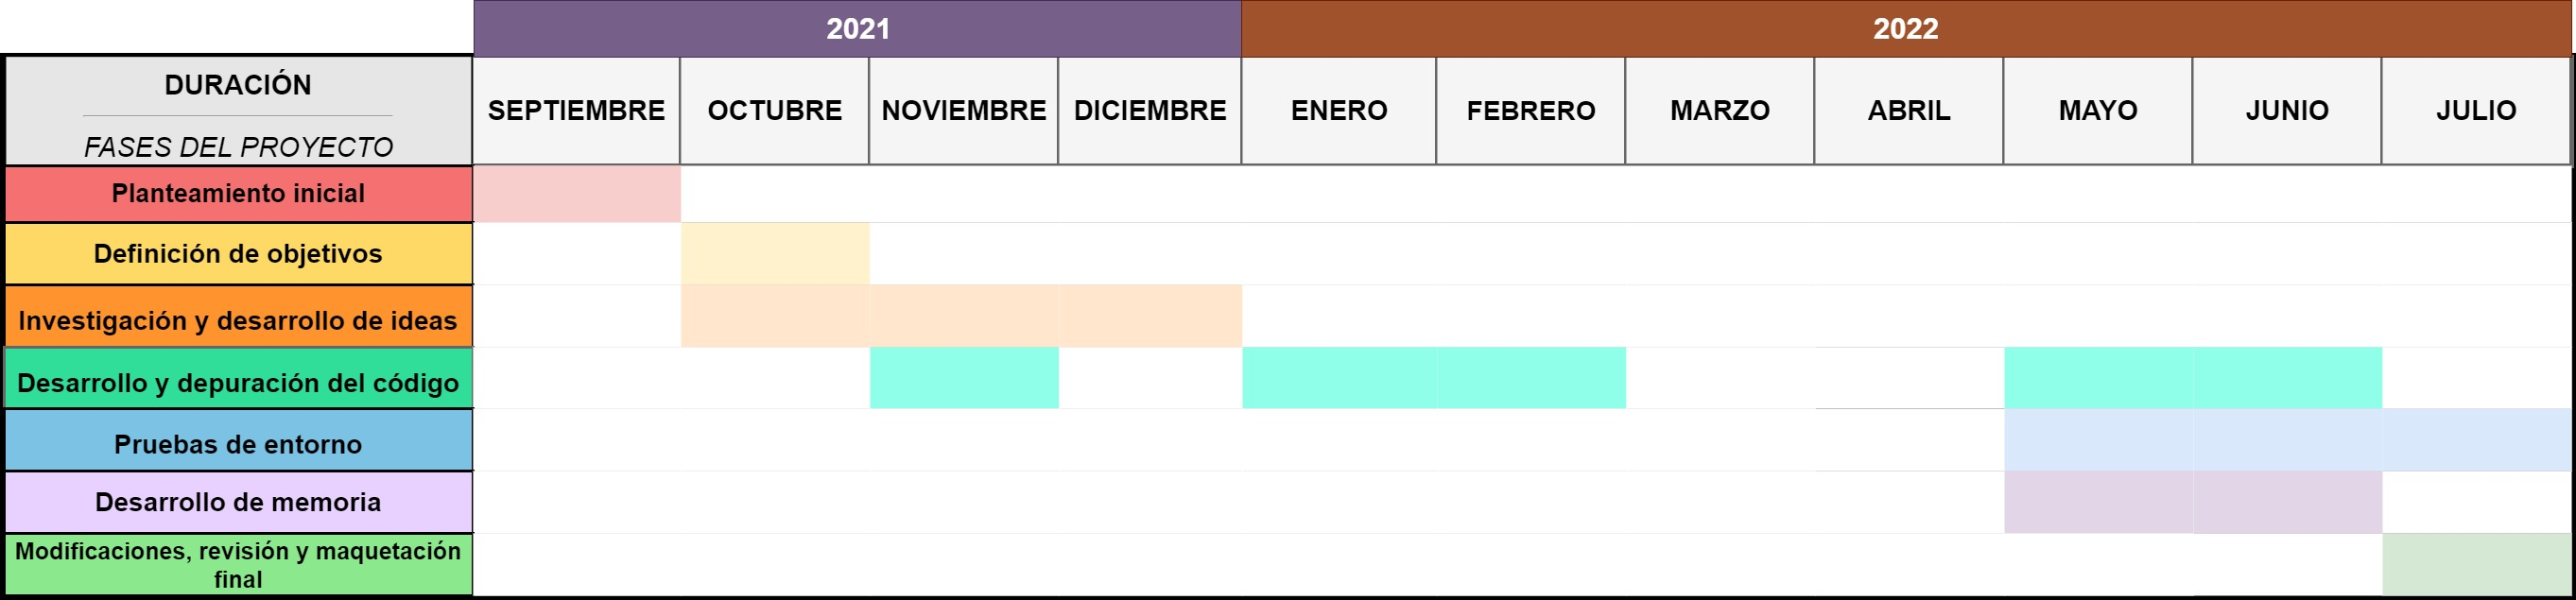
\includegraphics[width=16cm, keepaspectratio]{img/gantt.jpg}
    \caption{Diagrama de Gantt}
    \label{fig:diagrama_gantt}
\end{figure}

\pagebreak 
Para facilitar la organización, estructuración y consecución de objetivos se hace uso de la herramienta Trello\footnote{\url{https://trello.com/tfg_felipesandoval/boards}}, allí se dividen las tareas en tres bloques: \textbf{Investigativo} (Amarillo), \textbf{Desarrollo de código} (Verde) y \textbf{Desarrollo de memoria} (Rojo) 

 \begin{figure}[h]
 	 \centering
    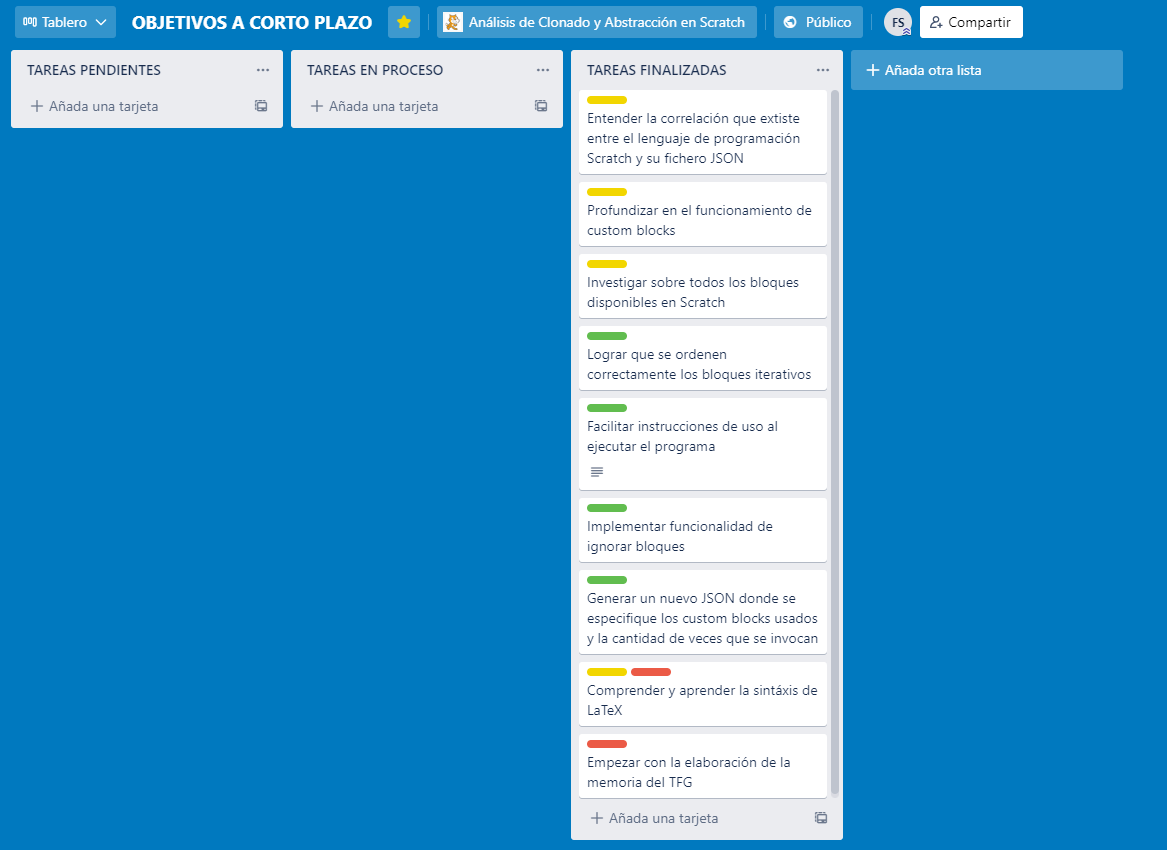
\includegraphics[width=15cm, keepaspectratio]{img/obj_cortoplazo.png}
    \caption{Tablero de Trello con objetivos a corto plazo}
    \label{fig:tableros_trello}
 \end{figure}

 \begin{figure}[h]
  	 \centering
    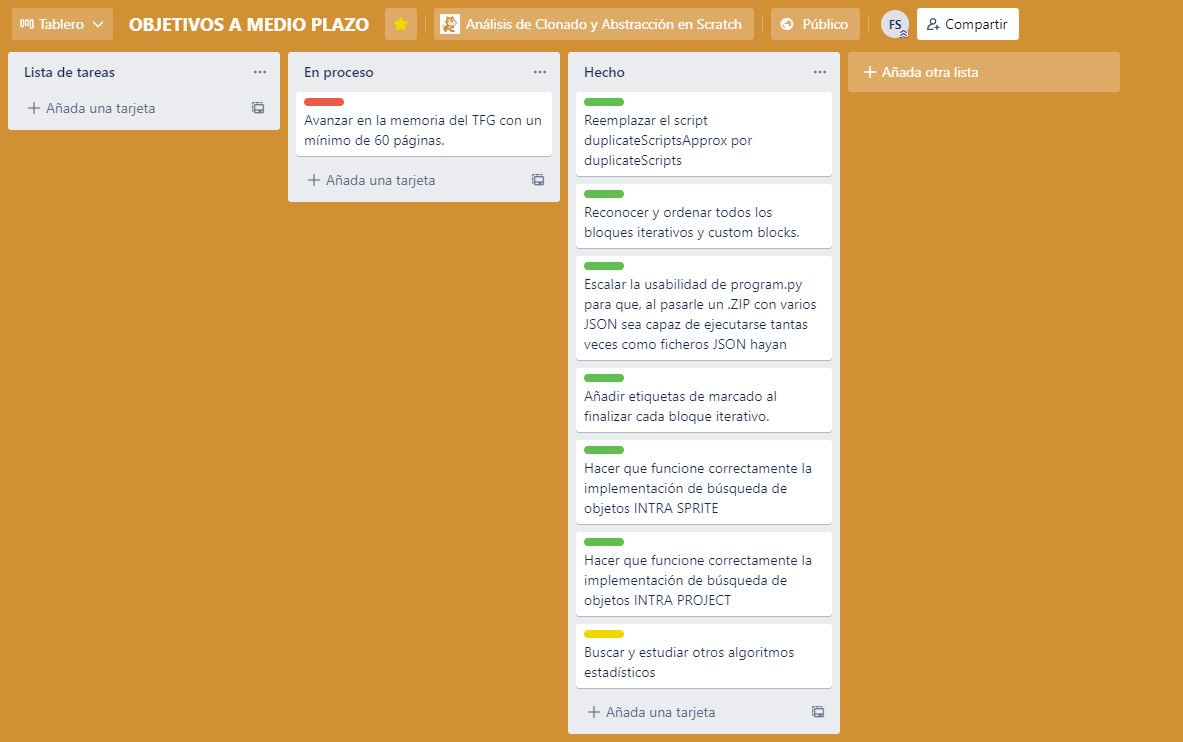
\includegraphics[width=15cm, keepaspectratio]{img/obj_medioplazo.png}
    \caption{Tablero de Trello con objetivos a medio plazo}
    \label{fig:tableros_trello}
 \end{figure}
 
  \begin{figure}[h]
  	 \centering
    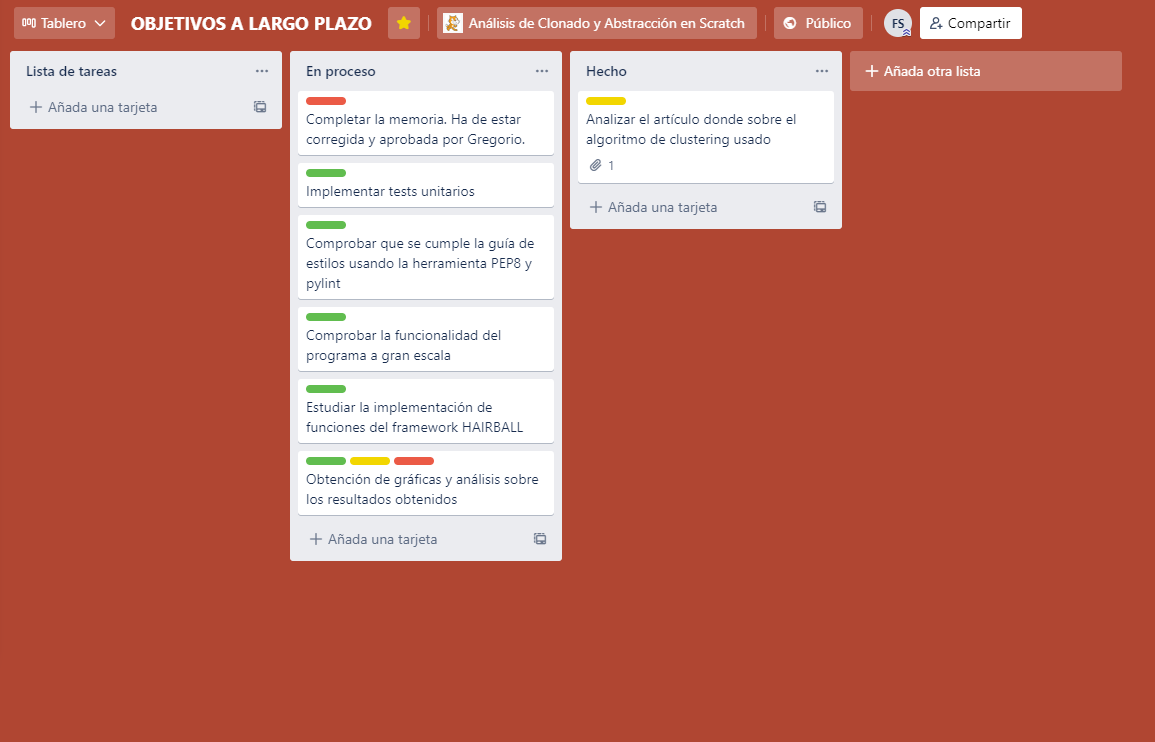
\includegraphics[width=15cm, keepaspectratio]{img/obj_largoplazo.png}
    \caption{Tablero de Trello con objetivos a largo plazo}
    \label{fig:tableros_trello}
 \end{figure}
 
%A continuación, viene una figura, la Figura~\ref{figura:foro_hilos}. 
%También habrás tomado nota de cómo se ponen las ``comillas dobles'' para que se muestren correctamente. 
%Nota que hay unas comillas de inicio (``) y otras de cierre (''), y que son diferentes.
%Volviendo a las referencias, nota que al compilar, la primera vez se crea un diccionario con las referencias, y en la segunda compilación se ``rellenan'' estas referencias. 
%Por eso hay que compilar dos veces tu memoria.
%Si no, no se crearán las referencias.

%%%%%%%%%%%%%%%%%%%%%%%%%%%%%%%%%%%%%%%%%%%%%%%%%%%%%%%%%%%%%%%%%%%%%%%%%%%%%%%%
%%%%%%%%%%%%%%%%%%%%%%%%%%%%%%%%%%%%%%%%%%%%%%%%%%%%%%%%%%%%%%%%%%%%%%%%%%%%%%%%
% ESTADO DEL ARTE %
%%%%%%%%%%%%%%%%%%%%%%%%%%%%%%%%%%%%%%%%%%%%%%%%%%%%%%%%%%%%%%%%%%%%%%%%%%%%%%%%

\cleardoublepage
\chapter{Estado del arte}
\label{chap:estado}

En este capítulo se introducen las bases tecnológicas del trabajo.

\section{Scratch}
\label{sec:Scratch}

Scratch es un lenguaje de programación creado por el Grupo Lifelong Kindergarten del Laboratorio de Medios del MIT. En scratch se permite programar historias interactivas, videojuegos, felicitaciones, animaciones; entre otros, todo esto a través de un entorno completamente visual que se fundamenta en el uso de personajes, escenarios y bloques gráficos que permiten interactuar entre estos elementos.

Entre sus cualidades desatacan que es totalmente gratuito, de uso libre, multilenguaje y altamente recomendado para la iniciación de niños y adolescentes en el mundo de la programación. Scratch es, además, una gran comunidad de usuarios de los que se puede aprender y compartir proyectos. Los mayores consumidores de Scratch en el mundo son Estados Unidos y Reino Unido donde los niños que más usan Scratch son los que tienen una edad media entre los 13 y los 16 años.

En Scratch, los objetos se denominan \textit{sprites} y la parte visual es construida por piezas de puzle llamadas \textit{blocks} que al encajar entre sí forman funciones, conocidas como \textit{scripts}. Existen varias categorías de bloques, siendo de especial interés las siguientes: 

\begin{itemize}
  	\item \underline{Movimiento}: Usados para mover y girar un objeto por la pantalla.
  	\item \underline{Apariencia}: Usados para cambiar la visualización de un objeto.
  	\item \underline{Sonido}: Usados para reproducir o detener secuencias de audio.
  	\item \underline{Eventos}: Usados para controlar eventos que ejecuten determinadas acciones.
  	\item \underline{Datos}: Usados para para crear y asignar variables.
  	\item \underline{Control}: Usados para crear bucles o condicionales de ejecución.
  	\item \underline{Custom blocks}: Bloques definidos por el usuario. A modo de comparativa, son funciones personalizadas que podrán ser invocadas a lo largo del código.
\end{itemize}

La forma de programar en Scratch permite al usuario aprender rápidamente sin tener que comprender la sintaxis del lenguaje, centrándose en la lógica del programa, lo que mejora la habilidad de abstracción del usuario. \cite{arotuma2017programacion}

\section{JSON}
\label{sec:Json}

JavaScript Object Notation, mejor conocido como JSON, es un formato ligero de intercambio de datos que puede ser leído por cualquier persona. Este tipo de ficheros almacena información estructurada que es utilizada principalmente para transferir datos entre un servidor y un cliente. \footnote{https://www.json.org/json-en.html}

Tomando como referencia la sintáxis, existen dos elementos centrales en un fichero JSON \textit{Keys y Values}. Las \textit{Keys} o llaves, contienen una secuencia de caracteres rodeados de comillas y los \textit{Values} o claves, son un tipo de datos JSON válido. Puede tener la forma de un array, un diccionario, un string, un boolean, un objeto, un número o de tipo nulo. 

Es importante mencionar el fichero JSON ya que contiene la información necesaria para el análisis de datos de mi proyecto en Scratch.

\section{Python}
\label{sec:Python}

Es un lenguaje de programación interpretado cuya filosofía hace énfasis en tener una sintaxis sencilla favorecedora al código legible. Se trata así de un lenguaje de programación multiparadigma, ya que soporta la programación orientada a objetos, la programación imperativa y la programación funcional. Python fue creado por Guido van Rossum a finales de los ochenta y su nombre se lo debe a los humoristas británicos \textit{“Monty Python”}. \footnote{https://platzi.com/blog/historia-python/}

Existen tres versiones principales de Python pero las más extendidas son las versiones 2 y 3, siendo la versión 3.10 la última actualización disponible. En este proyecto se hace un uso íntegro de la versión Python 3.9. Cabe recalcar que las versiones 2 y 3 son incompatibles entre sí por el gran número de diferencias que existen entre ellas.

De todos los lenguajes de programación que aprendí a lo largo de la carrera he elegido Python por ser un lenguaje con una sintaxis sencilla, por ser multiplataforma, por su código abierto y, especialmente, por ser fuertemente tipado, ya que facilita la depuración de código y minimiza errores durante su compilación y ejecución.

Este proyecto se apoya en una serie de bibliotecas y módulos de Python. A continuación se enumeran y detallan el funcionamiento de cada uno:

\subsection{Sys}
\label{sec:sys}

Módulo que permite interactuar con los parámetros y funciones específicas del sistema. Es usado para solicitar argumentos por consola y para detener la ejecución del programa mostrando un mensaje por pantalla. También es usado para la registrar información de los mensajes de error en el fichero de log de eventos.

\subsection{Os}
\label{sec:os}

Módulo que permite trabajar, de forma portátil, con las funcionalidades del sistema operativo. En este proyecto se usa para eliminar ficheros JSON una vez ya han sido analizados, esto a fin de evitar crear excesivos documentos por cada ejecución.

\subsection{Shutil}
\label{sec:os}

Módulo que ofrece varias operaciones de alto nivel en archivos y colecciones de archivos. Es usado para copiar ficheros dentro de la ruta donde se ejecute el script.

\subsection{ZipFile}
\label{sec:zipfile}

Módulo que permite el manejo de archivos con extensión de tipo ZIP. Se usa para abrir, descomprimir y extraer ficheros dentro de este tipo de contenedores.

\subsection{JSON}
\label{sec:jsonmodule}

Módulo que ofrece la posibilidad de manipular ficheros de tipo JSON. Es usado para \textit{parsear}\footnote{Proceso de analizar una secuencia de símbolos a fin de determinar su estructura gramatical definida. También llamado análisis de sintaxis.} los elementos del fichero JSON de cada proyecto Scratch.

\subsection{Logging}
\label{sec:logging}

Módulo que define funciones y clases para implementar un sistema de registro de eventos de log para aplicaciones y bibliotecas. Se usa para generar el fichero \textbf{program\_logs.txt} que mostrará información relevante de la ejecución del programa. Es en este fichero donde se escribirán errores de ejecución y se detallará sobre la causa del fallo.

\subsection{Traceback}
\label{sec:traceback}

Módulo que copia el comportamiento del intérprete de Python cuando muestra una traza de pila. Es usado para obtener información de fallos relevantes en el fichero de logging.

\subsection{difflib}
\label{sec:difflib}

Módulo que implementa clases y funciones que ayudan a computar y trabajar con diferencias entre secuencias. Es especialmente útil para comparar texto e incluyen funciones que usan diversos algoritmos para lograr obtener esta información.

\subsubsection{SequenceMatcher}
\label{sec:difflib_SequenceMatcher} 

Clase flexible que se usa para comparar pares de secuencias de cualquier tipo, siempre y cuando los elementos de la secuencia sean separables. Esta clase implementa un método heurístico que identifica automáticamente ciertos elementos como no deseados, para ello cuenta cuantas veces aparece cada elemento en la secuencia. Se usa para comparar secuencias en cadenas de caracteres.\footnote{https://towardsdatascience.com/sequencematcher-in-python-6b1e6f3915fc}

\subsection{collections}
\label{sec:collections}

Este módulo implementa tipos de datos que proporcionan alternativas a los contenedores integrados de uso general de Python, como diccionarios, listas, set, y tuplas.\footnote{https://docs.python.org/3/library/collections.html}

\subsubsection{counter}
\label{sec:difflib_counter}

Es una subclase del tipo de datos \textit{dict} para contar objetos separables. Los elementos se almacenan como llaves y sus conteos se almacenan como valores de diccionario. Se permite que los conteos sean cualquier valor entero, incluidos los conteos a cero o negativos.

\subsubsection{defaultdict}
\label{sec:difflib_defaultdict}

Es una subclase del tipo de datos \textit{dict} que anula un método y añade una variable de instancia editable a través de una función para suministrar valores faltantes. Funciona de forma parecida a los diccionarios clásicos de Python.

\subsubsection{ordereddict}
\label{sec:difflib_ordereddict}

Es una subclase del tipo de datos \textit{dict} que tiene métodos especializados para reorganizar el orden del diccionario ya que recuerda las entradas en el orden que se agregaron.

\subsection{sklearn}
\label{sec:sklearn}

Este módulo es usado para ejecutar funciones y clases de \textit{Machine Learning} construidas sobre SciPy. \footnote{https://scikit-learn.org/stable/modules/classes.html} Cuenta con algoritmos de clasificación, regresión, clustering y reducción de dimensionalidad. Además, es compatible con otras librerías de Python como NumPy y matplotlib.

\subsubsection{cluster}
\label{sec:sklearn_cluster}

Es una subclase que reúne diferentes algoritmos de agrupación no supervisada \textit{(unsupervised clustering)}. En este trabajo se hará uso del algoritmo \textbf{AffinityPropagation} ya que se evidencia que su uso es más óptimo en comparación con otros algoritmos. En la imagen \ref{fig:comparativa_algoritmos} se puede ver una comparativa visual sobre los distintos clasificadores de múltiples algoritmos. 

\begin{figure}[!h]
    \centering
    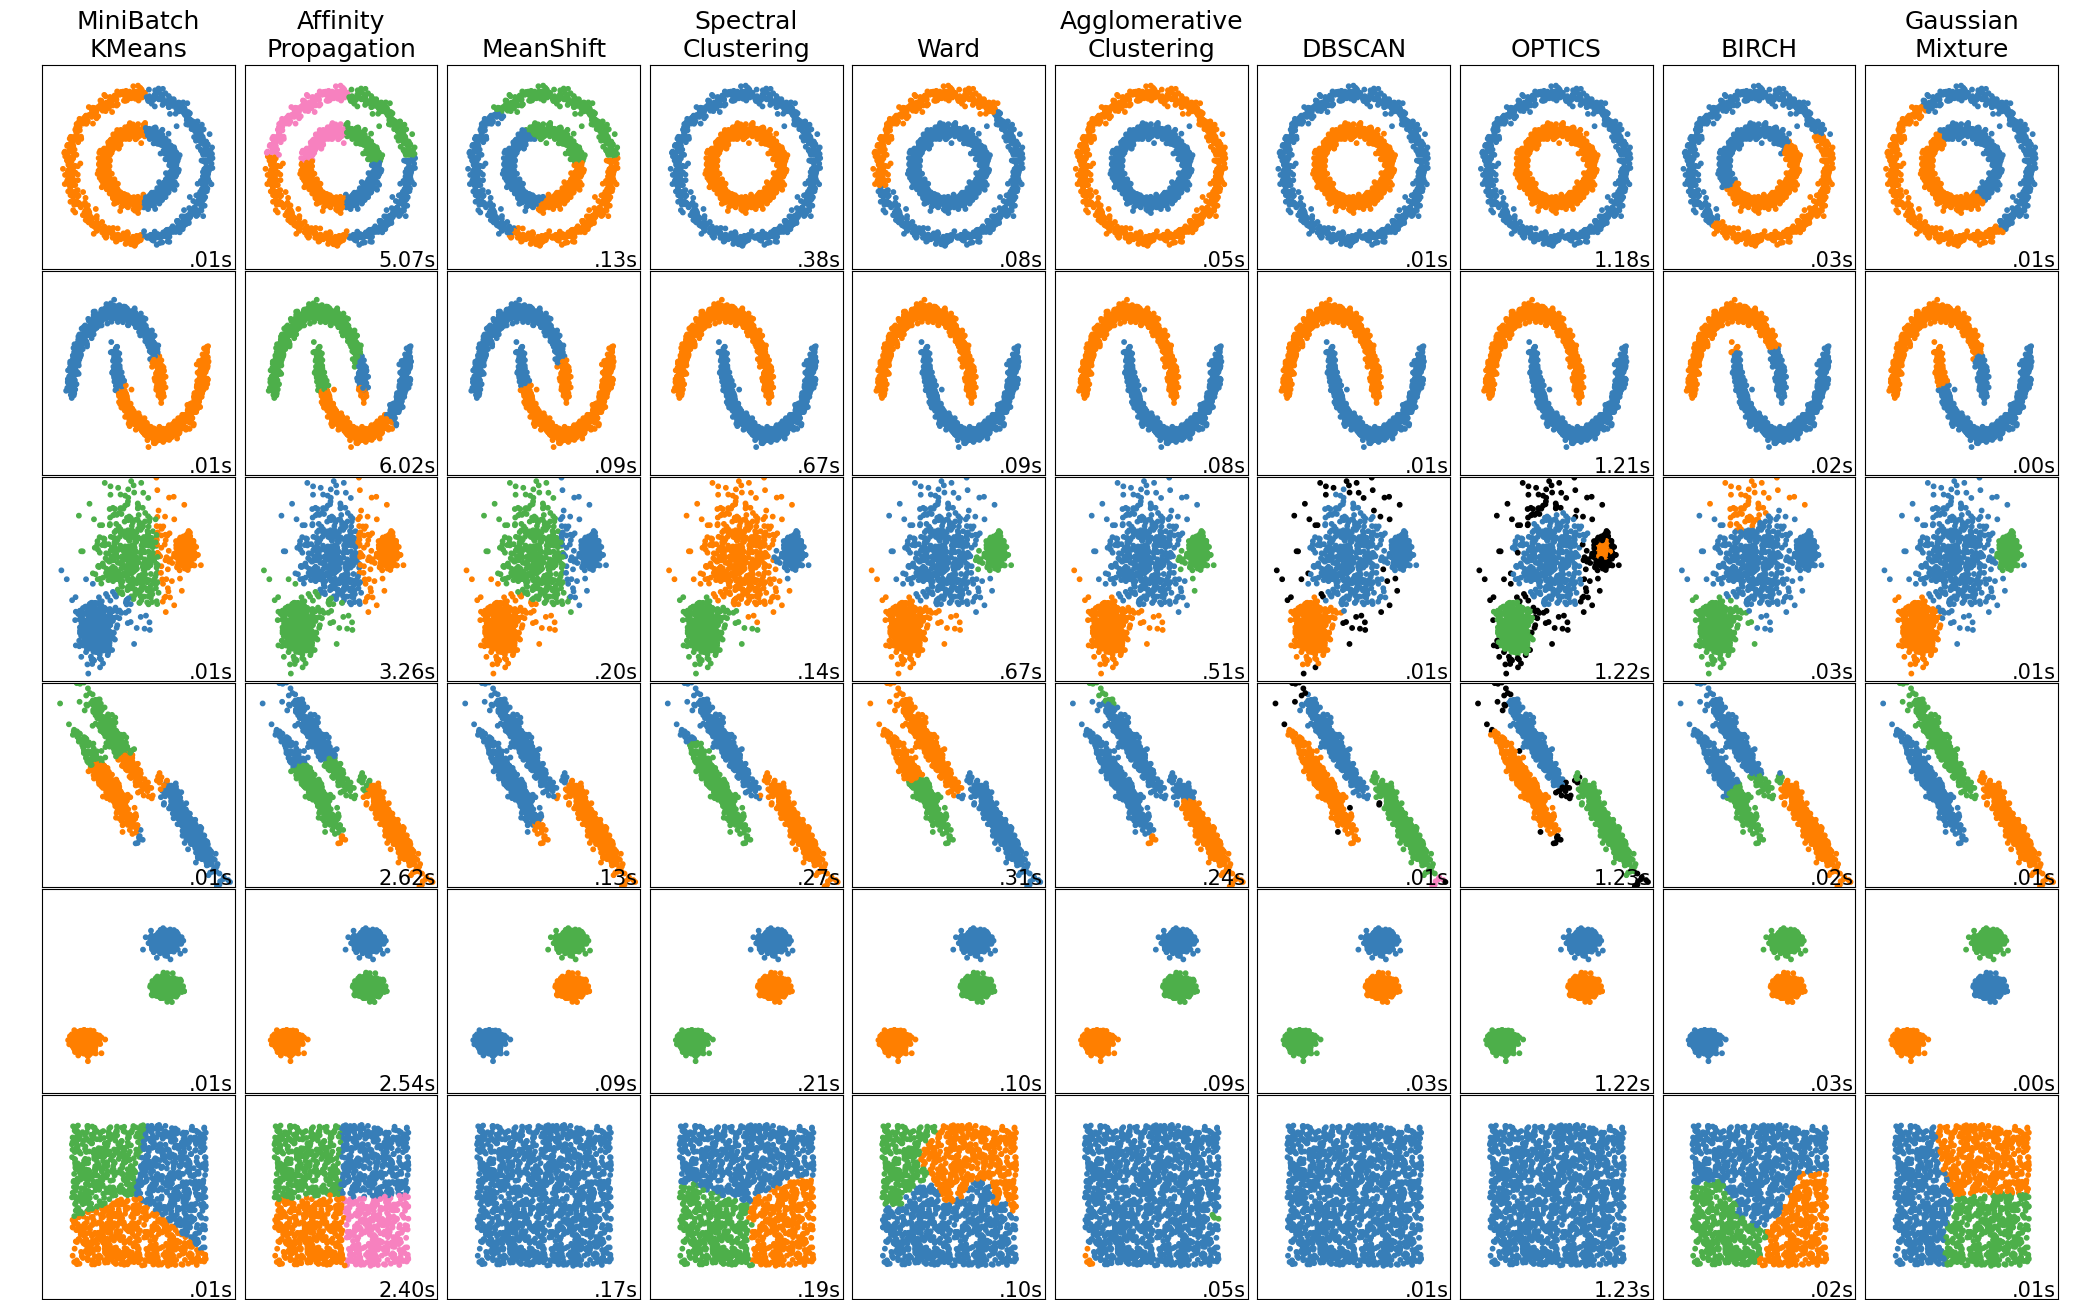
\includegraphics[width=16cm, keepaspectratio]{img/algorithm_comparison.png}
    \caption{Comparativa de algoritmos de clustering}
    \label{fig:comparativa_algoritmos}
\end{figure}

\section{Hairball} 
\label{sec:Hairball}

Hairball en un plugin de Python que analiza proyectos de Scratch, ofreciendo a su salida información acerca del nivel de habilidades del pensamiento computacional, como abstracción, paralelismo, lógica, sincronización, control de flujo, interactividad con el usuario y representación de los datos.

El modulo hairball permite generar una representacion en formato de grafo de los datos de un programa en Python. Esto es útil para visualizar el flujo de datos y el funcionamiento del programa.

También otorga información sobre malos hábitos de programación cómo código duplicado, código muerto, mal nombrado e inicialización de variables.\footnote{https://pypi.org/project/hairball/}

\section{Pip} 
\label{sec:pip}

Pip es un gestor de paquetes para el ecosistema de Python que es capaz de instalar y administrar paquetes mediante línea de comandos. Es el gestor con el que se han instalado todos los módulos y bibliotecas que no trae por defecto Python. Pip suele estar incluido al instalar Python, sin embargo, podría no ser así por lo que sería necesario su descarga. \footnote{https://pypi.org/project/pip/}

\section{Unittest} 
\label{sec:unittest}

Unittest es una herramienta empleada para realizar tests en Python, tanto para clases y módulos enteros como para scripts. Creada por Kent Beck, permite la automatización de tests y la opción de crear colecciones. Además, no está ligada a ningún marco de reportes por lo que nos permite utilizar el mas conveniente. Para todo lo mencionado Unittest se sirve de tests fixtures, test cases, test suites y test runner, propios de la programación orientada a objetos, conceptos explicados a continuación. 

\begin{itemize}
	\item \textbf{Test fixture}: es la preparación del entorno de todas las características del test que queremos ejecutar.
	\item \textbf{Test case}: es la unidad individual del test, nos permite generar un test unitario para testear cada función.
	\item \textbf{Test suite}: es la colección de los test cases que se ejecutan y agrupan juntos, también puede existir una coleccion de test suites. Ejecutar una suite es lo mismo que ejecutar una serie de test cases individualmente.
	\item \textbf{Test runner}: es el componente encargado de ejecutar los tests y proporcionar un resultado. Puede disponer de una interfaz gráfica, texto o devolver un valor especial.
\end{itemize}
 
Para ejecutar el conjunto de test desarrollados en este proyecto es necesario ejecutar la siguiente orden en línea de comandos:

\begin{lstlisting}[style=consola,numbers=none]
$ python3 -m unittest discover
\end{lstlisting}

\section{Guía de estilo PEP8} 
\label{sec:pep8}

PEP8 (Python Enhancement Proposal 81) es una guía de estilos definida para Python. Se trata de un conjunto de recomendaciones cuyo objetivo es ayudar a escribir código de forma estándar y legible. Es la guía de estilo elegida porque se usó durante la elaboración de prácticas de la asignatura Protocolos de Transmisión de Audio y Vídeos por Internet (PTAVI). Algunas de las reglas mas importantes de esta guía son:

\begin{itemize}
	\item Indentación en cuatro espacios.
	\item Espacios antes de cada tabulación.
	\item Líneas limitadas a 79 caracteres.
	\item Saltos de línea con barra invertida.
\end{itemize}

Actualmente, la herramienta ha sido renombrada como \textit{pycodestyle} y el comando de instalación necesario es el siguiente:

\begin{lstlisting}[style=consola,numbers=none]
$ pip install pycodestyle
\end{lstlisting}

%%%%%%%%%%%%%%%%%%%%%%%%%%%%%

%Hemos hablado de cómo incluir figuras.
%Pero no hemos dicho nada de tablas.
%A mí me gustan las tablas.
%Mucho.
%Aquí un ejemplo de tabla, la Tabla~\ref{tabla:ejemplo} (siento ser pesado, pero nota cómo he puesto la referencia).

%\begin{table}
% \begin{center}
%  \begin{tabular}{ | l | c | r |} % tenemos tres colummnas, la primera alineada a la izquierda (l), la segunda al centro (c) y la tercera a la derecha (r). El | indica que entre las columnas habrá una línea separadora.
%    \hline
%    Uno & 2 & 3 \\ \hline % el hline nos da una línea vertical
%    Cuatro & 5 & 6 \\ \hline
%    Siete & 8 & 9 \\
%    \hline
%  \end{tabular}
%  \label{tabla:ejemplo}
%  \caption{Ejemplo de tabla. Aquí viene una pequeña descripción (el \emph{caption}) del contenido de la tabla. Si la tabla no es autoexplicativa, siempre viene bien aclararla aquí.}
% \end{center}
%\end{table}

%%%%%%%%%%%%%%%%%%%%%%%%%%%%%%%%%%%%%%%%%%%%%%%%%%%%%%%%%%%%%%%%%%%%%%%%%%%%%%%%
%%%%%%%%%%%%%%%%%%%%%%%%%%%%%%%%%%%%%%%%%%%%%%%%%%%%%%%%%%%%%%%%%%%%%%%%%%%%%%%%
% DISEÑO E IMPLEMENTACIÓN %
%%%%%%%%%%%%%%%%%%%%%%%%%%%%%%%%%%%%%%%%%%%%%%%%%%%%%%%%%%%%%%%%%%%%%%%%%%%%%%%%

\cleardoublepage
\chapter{Diseño e implementación}

En este capítulo se realiza una descripción detallada de la estructura del software desarrollado y la funcionalidad a nivel de código. También se indica el hilo de ejecución, el entorno de trabajo y las herramientas usadas para la consecución de este proyecto.

\section{Entorno y herramientas de trabajo} 
\label{sec:entorno}

Para poder obtener resultados confiables en múltiples entornos, se compila, ejecuta y depura el código en los sistemas operativos Windows e UNIX. Se hace uso de tres aplicaciones para mantener sincronizados ficheros, control de versiones y llevar un control sobre el planteamiento y la consecución de objetivos:

\begin{itemize}
  \item \textbf{Trello:} Es usada para gestionar y organizar, a modo de tableros, las fases y tareas por realizar tanto a corto, medio y largo plazo. 
  \item \textbf{Dropbox:} Herramienta empleada como servicio de almacenamiento en la nube para mantener sincronizados ficheros, imágenes y referencias de la memoria.
  \item \textbf{Github:} Es usada para alojar el código y mantener un control de versiones. Resulta muy útil para dar marcha atrás en caso de errores detectados mientras se avanza en la práctica, esto gracias al seguimiento de los cambios en el código
\end{itemize}

En el diagrama de flujo de la imagen \ref{fig:diagrama_trabajo} se muestra el entorno y las herramientas usadas.

 \begin{figure}[!h]
    \centering
    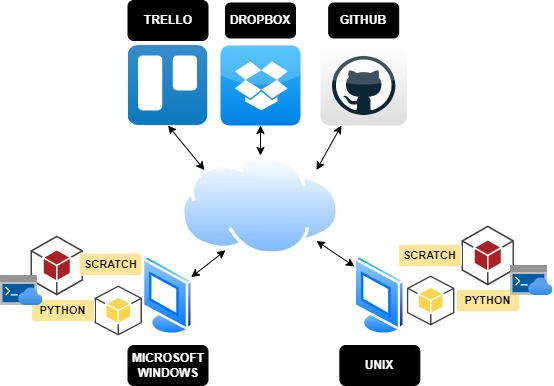
\includegraphics[width=9cm, keepaspectratio]{img/workplace.jpg}
    \caption{Diagrama de entorno y aplicaciones}
    \label{fig:diagrama_trabajo}
 \end{figure}

\section{Arquitectura general} 
\label{sec:arquitectura}

%Aquí viene todo lo que has hecho tú (tecnológicamente). Puedes entrar hasta el detalle.  Es la parte más importante de la memoria, porque describe lo que has hecho tú. Eso sí, normalmente aconsejo no poner código, sino diagramas.

%Si tu proyecto es un software, siempre es bueno poner la arquitectura (que es cómo se estructura tu programa a ``vista de pájaro'').

A nivel general, el flujo del funcionamiento del programa es el que se puede apreciar en la imagen \ref{fig:fasedesejecucion}. El script a ejecutar es \textit{program.py} y de allí se irán concatenando llamadas a los siguientes scripts, \textit{duplicatescripts.py}, \textit{most\_frequent\_blocks.py}, \textit{statistics.py} y finalmente, \textit{cluster.py}

\begin{figure}
  \centering
  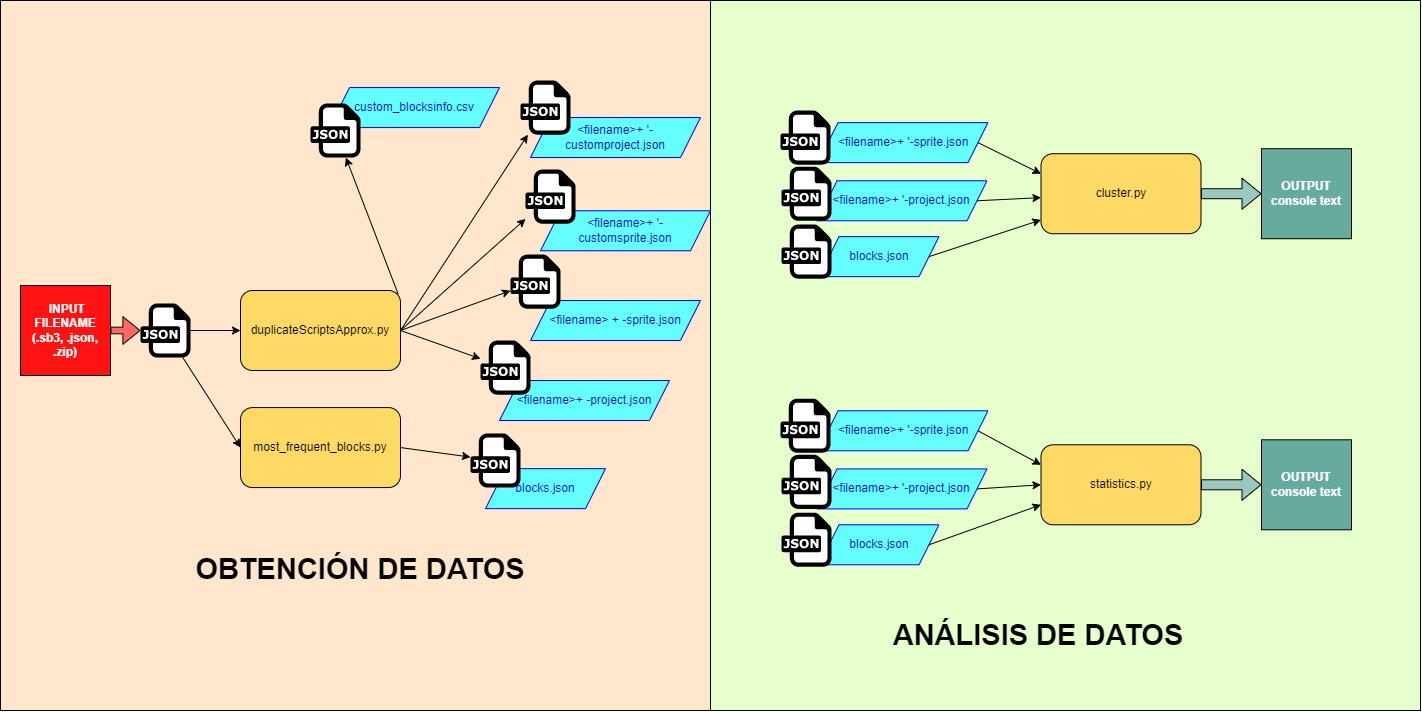
\includegraphics[width=15cm, keepaspectratio]{img/flow.jpg}
  \caption{Fase de extracción de datos}
  \label{fig:fasedesejecucion}
\end{figure}

Para ejecutar el software es necesario que el usuario pase por línea de comandos hasta un máximo de dos argumentos. Primero y obligatoriamente, el nombre del archivo a examinar, segundo y de forma opcional, el argumento \textbf{-i} que, de indicarlo, ignorará los bloques indicados en el fichero \textit{IgnoreBlocks.txt}. En caso de pasar más argumentos, el programa mostrará un mensaje de error y creará un fichero de registros en el que se escribirán los eventos que ocurran durante la ejecución.

Los ficheros a analizar pueden estar en formato SB3 (extensión que emplea Scratch) en formato JSON o un fichero comprimido en formato ZIP. El software se ha desarrollado para ser escalable, por lo que, para realizar un análisis extensivo de muchos proyectos, es necesario comprimir los ficheros JSON en un archivo ZIP. 

A continuación, se detallan los scripts, funciones y clases relevantes del software desarrollado.

\subsection{program.py}

Sirve como script principal. Su tarea principal es servir de hilo de ejecución de todo el programa, para ello extrae y parsea el contenido de ficheros JSON. En este programa se declara la forma como se escribirán los registros de control de ejecuciones en el archivo de logs, \textit{program\_logs.txt}, útil para depurar y encontrar excepciones durante la ejecución.

\subsection{duplicateScripts.py}

Este programa toma como argumentos el nombre del fichero con su extensión correspondiente, el contenido del archivo JSON y el argumento opcional que indica si se ignorará, o no, ciertos tipos de bloques.

El contenido del JSON se recorrerá a modo de diccionario, empezando por la clave \textit{targets} que contiene todos los objetos. Seguidamente se extrae la información relevante, según cada bloque, de la clave \textit{blocks}. En el código se irá almacenando, en una variable de tipo diccionario, la clave/valor: \textit{block\_id:opcode}, lo cual será importante para encontrar y añadir, en su posición correcta, a los bloques de control y personalizados. En la imagen \ref{fig:arboljson} se aprecia una vista de árbol general de las clave/valor del fichero JSON, y en la imagen \ref{fig:graljson} un diagrama de la estructura general de un bloque genérico.

\begin{figure}[!htb]
  \centering
  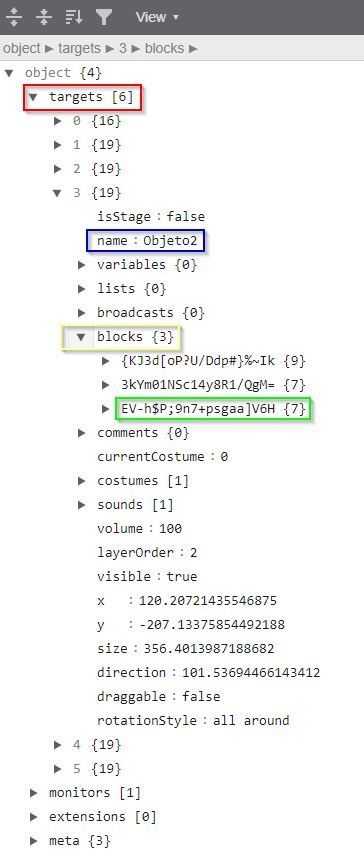
\includegraphics[width=7cm, keepaspectratio]{img/jsontree.jpg}
  \caption{Vista de árbol del contenido de un fichero JSON}
  \label{fig:arboljson}
\end{figure}

\begin{figure}[!htb]
  \centering
  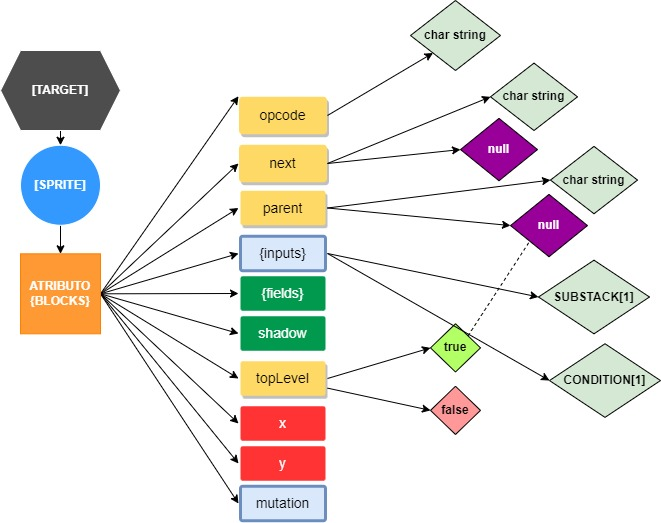
\includegraphics[width=17cm, keepaspectratio]{img/block_general.jpg}
  \caption{Estructura general de un bloque genérico}
  \label{fig:graljson}
\end{figure}


Todas las categorías de bloques suelen tienen una estructura similar pero no todos sus campos son relevantes. Las claves como \textbf{opcode}, \textbf{parent}, \textbf{next} y \textbf{topLevel} son esenciales para la organización y extracción de datos. Otras claves, como \textbf{inputs} y \textbf{mutation} no aparecen en todos los tipos de bloques, sin embargo, son igualmente imprescindibles para obtener el orden correcto en el conjunto de scripts. Es importante enfatizar que el \textit{Block\_ID} es un valor único por bloque, totalmente independiente del \textit{opcode}. A continuación, se enumeran los casos genéricos y particulares considerados:

\begin{enumerate}
\item Si el valor de \textbf{topLevel} es True significa que el elemento es el primer bloque de mi script. En este caso el valor de la clave \textbf{parent} es null. 
\item Si el valor de \textbf{topLevel} es False significa que el elemento no es el primer bloque. En este caso el valor de la clave \textbf{parent} contiene el \textit{Block\_ID} del bloque superior.
\item La clave de \textbf{opcode} siempre tendrá como valor un string con el nombre de ese bloque.
\item El valor de \textbf{next} puede ser un string con el \textit{Block\_ID} del siquiente bloque o puede ser null. En este último caso, puede ser porque es el último elemento del script, porque es un bloque de control (control\_repeat, control\_forever) o porque es un bloque definido por el usuario (custom\_block). En la imagen \ref{fig:loopsforever} se puede ver un ejemplo de esto.
\item Dentro del valor \textbf{inputs} se encuentra otra clave llamada \textbf{substack} que contiene los elementos internos de los bloques de control (control\_repeat, control\_forever, control\_if, control\_repeat\_until y control\_if\_else). Este valor es exclúsivo de este tipo de bloques. En las imagenes \ref{fig:controlblock} y \ref{fig:scratch_control} se ejemplifican estos casos.
\item Para el caso especial del bloque control\_if\_else el valor \textbf{substack2} contiene otra lista con la secuencia de bloques internas en el hilo condicional. En la imagen \ref{fig:controlblock_spe} se puede ver un ejemplo de la estructura del JSON y en la imagen \ref{fig:scratch_special} un script y sus elementos.
\item Se añaden las siguientes marcas de control al finalizar los siguientes bloques:
\begin{itemize}
\item Marca ''END\_IF'' al final de la primera condición de los bloques control\_if, control\_repeat\_until y control\_if\_else
\item Marca ''END\_ELSE'' al final de la segunda condición del bloque control\_if\_else
\item Marca ''END\_LOOP'' al final de todos los bloques de control
\end{itemize}
\end{enumerate}

\begin{figure}
  \centering
  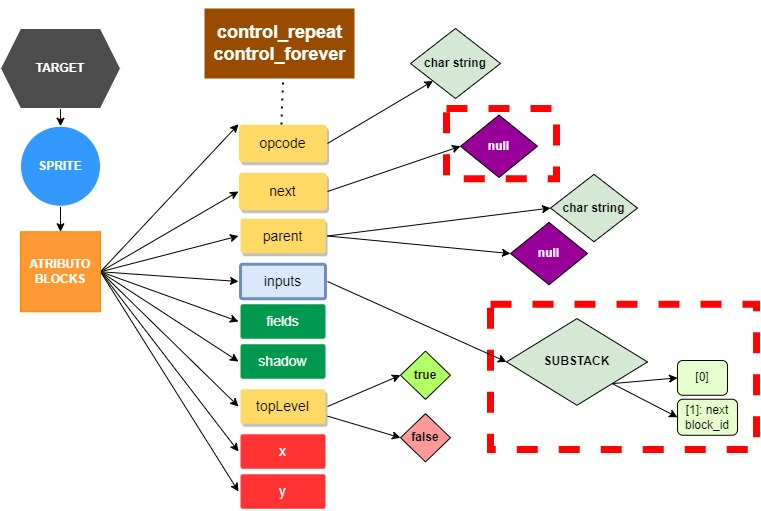
\includegraphics[width=15cm, keepaspectratio]{img/block_loop.jpg}
  \caption{Estructura general de un bloque de tipo control\_repeat y control\_forever}
  \label{fig:loopsforever}
\end{figure}

\begin{figure}
	\centering
  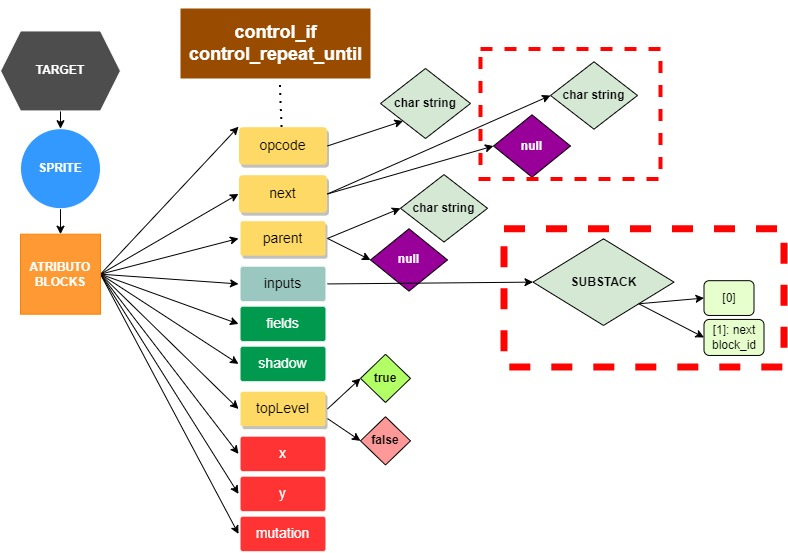
\includegraphics[width=15cm, keepaspectratio]{img/block_controlif.jpg}
  \caption{Estructura de un bloque condicional de tipo control\_if o control\_repeat\_until}
  \label{fig:controlblock}
\end{figure}

\begin{figure}
  \centering
  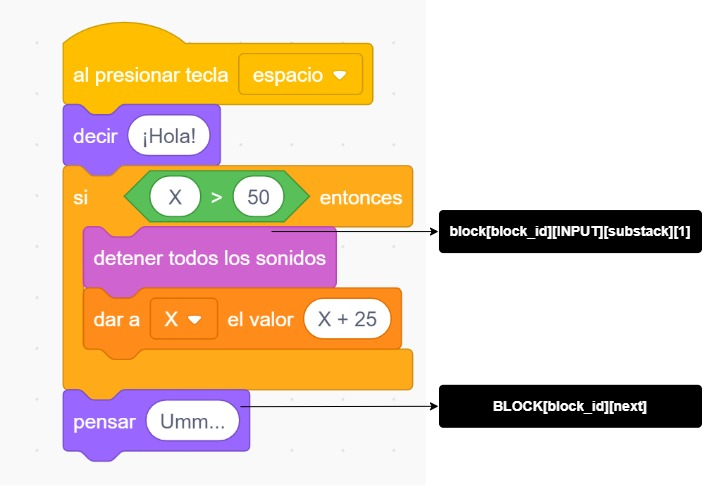
\includegraphics[width=13cm, keepaspectratio]{img/scratch_control.jpg}
  \caption{Script con bloques de control}
  \label{fig:scratch_control}
\end{figure}

\begin{figure}
  \centering
  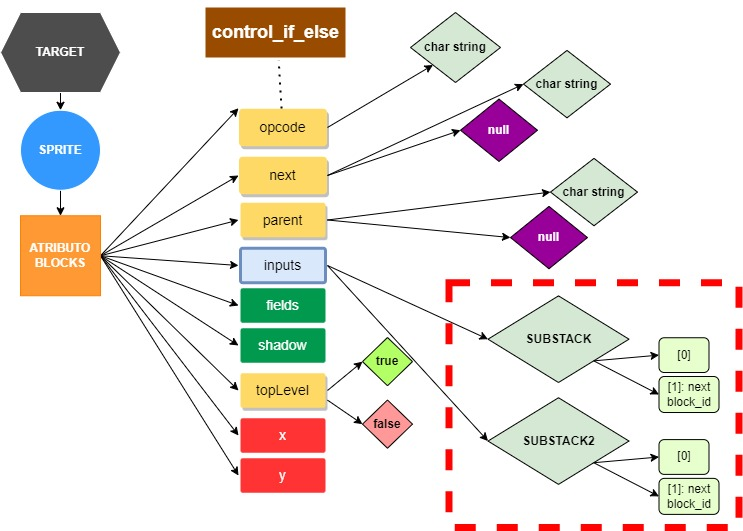
\includegraphics[width=15cm, keepaspectratio]{img/controlblock_spe.jpg}
  \caption{Estructura general de un bloque condicional de tipo control\_if\_else}
  \label{fig:controlblock_spe}
\end{figure}

\begin{figure}
  \centering
  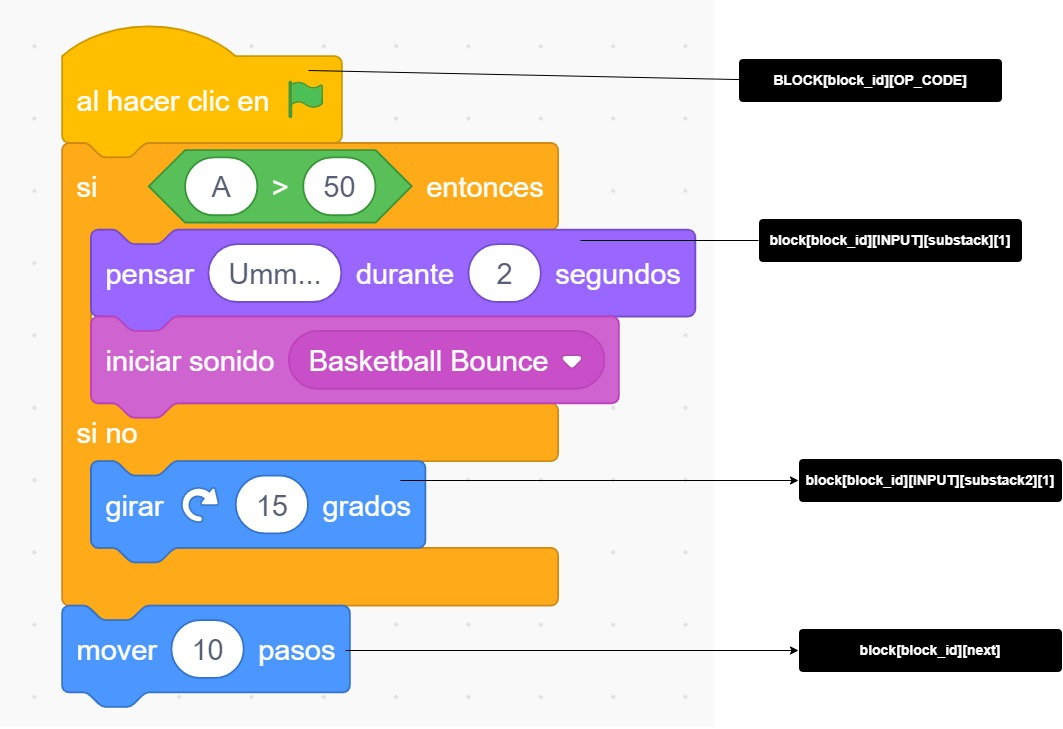
\includegraphics[width=13cm, keepaspectratio]{img/scratch_special.jpg}
  \caption{Script con bloque condicional de tipo control\_if\_else}
  \label{fig:scratch_special}
\end{figure}

\newpage 
Para los bloques personalizados por el usuario, los \textit{custom\_blocks}, se tienen en cuenta los tres siguientes casos:

\begin{enumerate}
\item Para elementos con \textbf{opcode} cuyo valor sea \textit{procedures\_prototype}:
\begin{itemize}
\item Su clave \textbf{next} tendrá siempre null como valor.
\item Su clave \textbf{parent} tiene como valor el block\_ID de \textit{procedures\_definition}.
\item Su clave \textbf{topLevel} tendrá siempre false como valor.
\item En su clave \textbf{mutation} se encuentra tanto el nombre de la función, como los argumentos y sus respectivos valores.
\end{itemize}

\item Para elementos con \textbf{opcode} cuyo valor sea \textit{procedures\_definition}:
\begin{itemize}
\item Su clave \textbf{parent} tendrá siempre null como valor.
\item Su clave \textbf{topLevel} tendrá siempre true como valor.
\item En su clave \textbf{inputs} se encuentra la sucesión de bloques que conforman mi custom block.
\end{itemize}

\item Para elementos con \textbf{opcode} cuyo valor sea \textit{procedures\_call}:
\begin{itemize}
\item En su clave \textbf{mutation} se encuentra el nombre de la función lo que permitirá contabilizar el número de llamadas que se hagan.
\end{itemize}
\end{enumerate}

\begin{figure}[!htb]
  \centering
  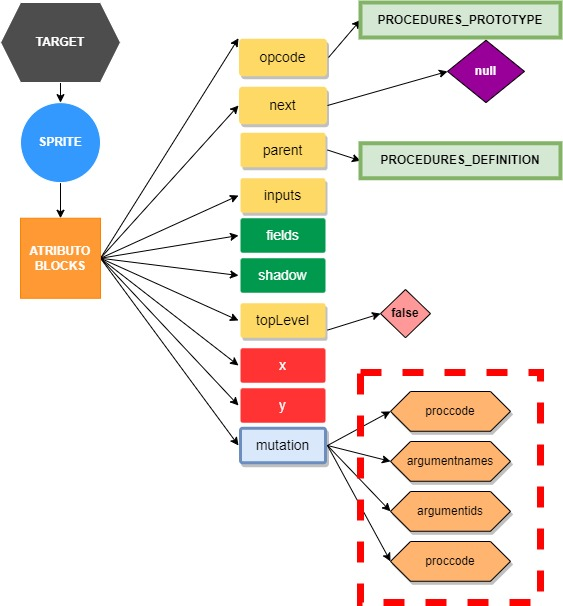
\includegraphics[width=13cm, keepaspectratio]{img/block_prototype.jpg}
  \caption{Estructura general de un bloque de tipo block\_prototype}
  \label{fig:controlblock_spe}
\end{figure}

\begin{figure}[!htb]
  \centering
  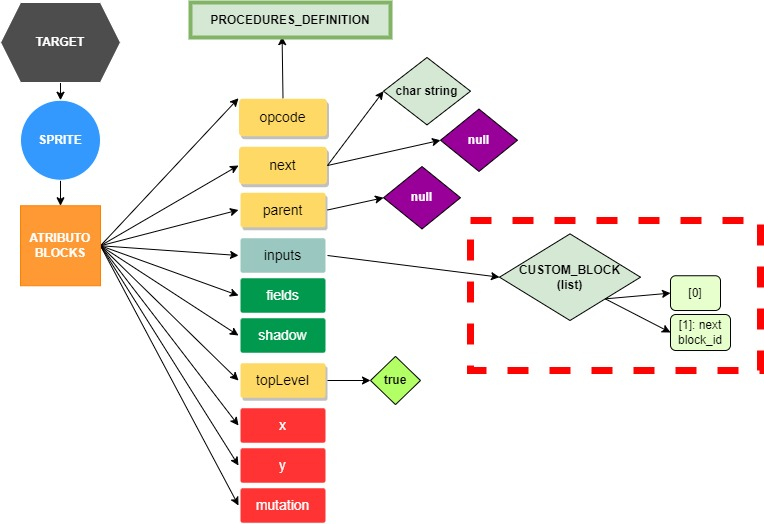
\includegraphics[width=15cm, keepaspectratio]{img/block_definition.jpg}
  \caption{Estructura general de un bloque de tipo block\_definition}
  \label{fig:controlblock_spe}
\end{figure}

\begin{figure}[!htb]
  \centering
  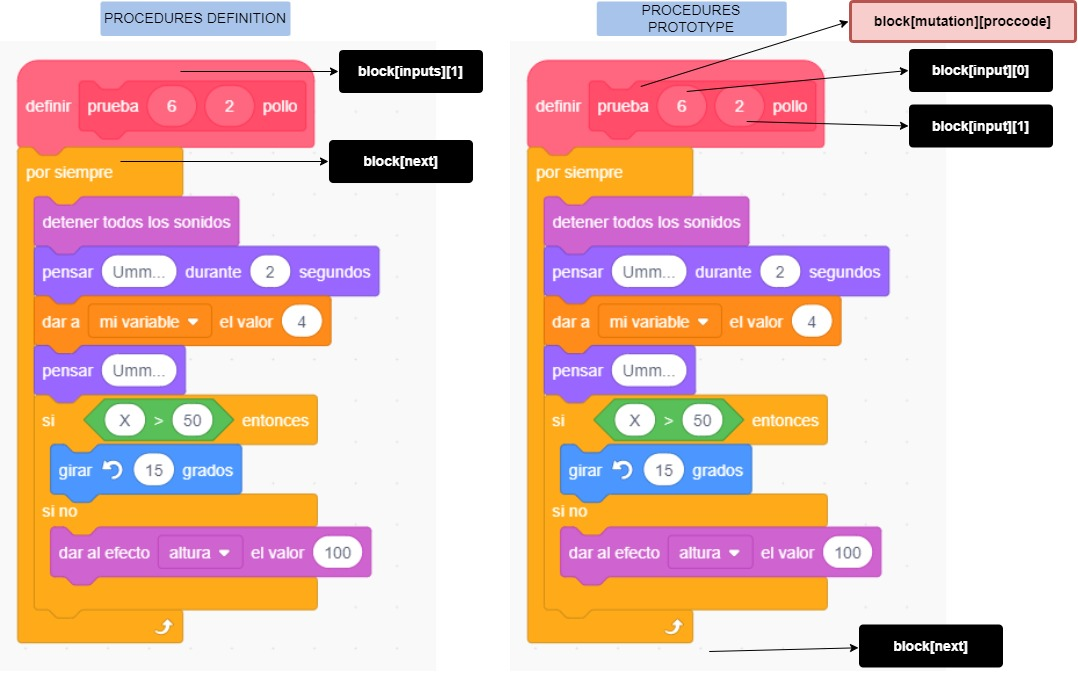
\includegraphics[width=13cm, keepaspectratio]{img/scratch_custom.jpg}
  \caption{Diferencias entres los bloques custom\_block}
  \label{fig:scratch_special}
\end{figure}

\newpage 
Uno de los principales problemas al momento de analizar el JSON ha sido ordenar de forma correcta la estructura de bloques, ya que por defecto no se muestran de forma ordenada. Para lograrlo se crean dos diccionarios: \textit{scripts\_dict} que almacena como valor los bloques de cada sprite y, en el otro diccionario \textit{self.blocks\_dict} que almacena como clave el block\_id de cada bloque y como valor su opcode. Además, este último es vital para insertar bloques según el block\_id del parent que le corresponda.

Una vez se tiene todos los bloques de cada sprite ordenados, se procede a obtener los bloques duplicados. Esto se logra gracias a la función \textbf{find\_dups}, que toma como argumento una lista de bloques. Puede ser, exclusiva para los bloques de cada objeto(\textit{intra-sprite})o para todos los bloques del proyecto (\textit{wide-project}). La función hace uso de la clase sequenceMatcher para comparar, palabra a palabra, cada bloque entre sí y devolver una lista con los bloque que mas se repitan. 

% IMAGEN DE CODIGO, MEJOR NO.
%\begin{figure}
%  \centering
%  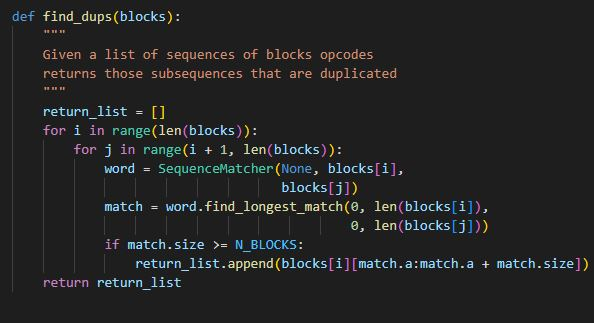
\includegraphics[width=13cm, keepaspectratio]{img/code_dups.jpg}
%  \caption{Código de la función find\_dups}
%  \label{fig:code_finddups}
%\end{figure}

\section{Obtención de datos} 
\label{sec:obtenciondatos}

Para finalizar la ejecución de \textbf{duplicateScripts.py}, se ejecuta la función \textbf{finalize} se genera tres ficheros de tipo JSON. En la imagen \ref{fig:flow_finddups} se puede apreciar un diagrama acerca la última fase de ejecución de este script.

\begin{itemize}
\item ''filename''-sprite.json: Contendrá las cadena de bloques mas repetidos por objeto.
\item ''filename''-project.json: Contendrá las cadena de bloques mas repetidos en todo el programa.
\item ''filename''-custom.json: Contendrá las cadena de bloques personalizados mas repetidos en todo el programa.
\end{itemize}

\begin{figure}[!htb]
  \centering
  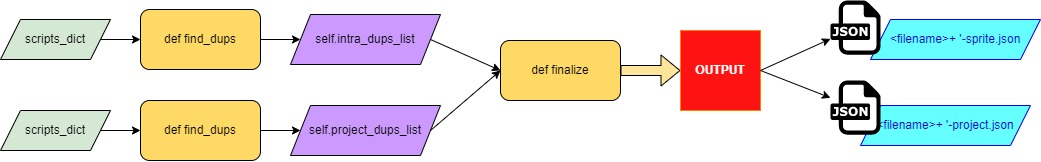
\includegraphics[width=15cm, keepaspectratio]{img/flow_finddups.jpg}
  \caption{Diagrama de la última fase de ejecución duplicateScripts.py}
  \label{fig:flow_finddups}
\end{figure}

\subsection{most\_frequent\_blocks.py}

Este script toma como argumento un fichero JSON, e itera sobre sus elementos para buscar y contabilizar los \textit{opcodes} de los bloques que más se repiten. Luego, ordena los bloques por frecuencia de uso y los guarda en un nuevo archivo JSON: \textbf{blocks.json}. Se le asignara un caracter a cada bloque según su frecuencia de repetición. Al bloque mas repetido le corresponde la primera letra del abecedario y así sucesivamente completando la cadena de caracteres definida en la variable \textit{characters}. Se puede apreciar el diagrama del funcionamiento del   en la imagen \ref{fig:flow_mostfreq}


%\begin{figure}
%  \centering
%  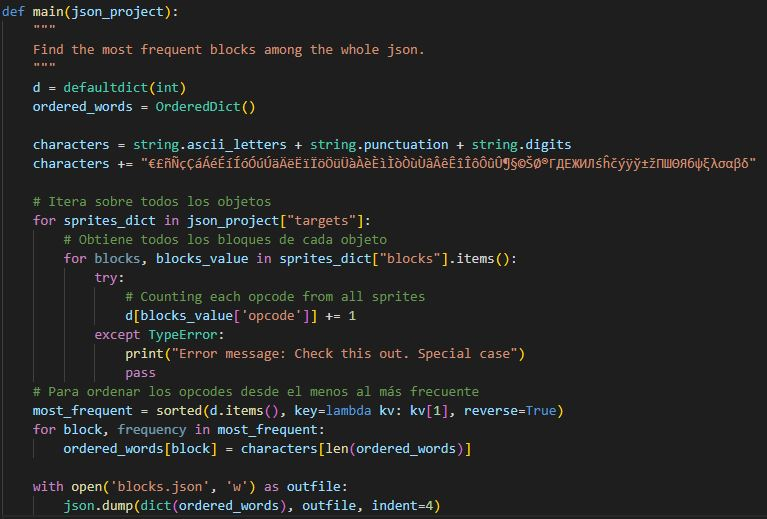
\includegraphics[width=13cm, keepaspectratio]{img/code_mostfrequent.jpg}
%  \caption{Código del script most\_frequent\_blocks.py}
%  \label{fig:code_mostfrequent}
%\end{figure}

\begin{figure}[!htb]
  \centering
  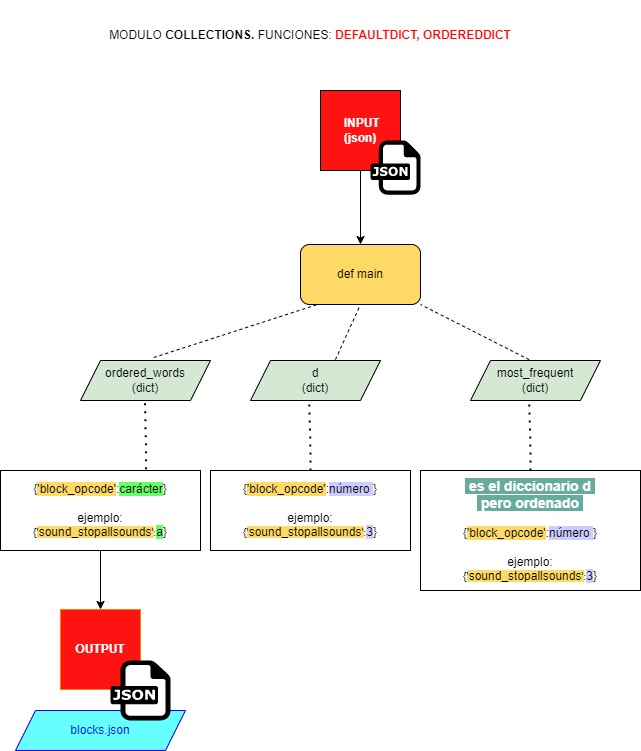
\includegraphics[width=15cm, keepaspectratio]{img/flow_mostfreq.jpg}
  \caption{Diagrama de funcionamiento de most\_frequent\_blocks.py}
  \label{fig:flow_mostfreq}
\end{figure}

\newpage 

\section{Procesado de datos} 
\label{sec:procesadodatos}

\subsection{statistics.py}

Este script analiza los ficheros JSON generados por el código de \textbf{duplicateScripts.py} con ayuda de los módulos \textit{counter}, \textit{defaultdict} y \textit{json}. Luego, la función \textbf{json2dna} carga el contenido del fichero \textbf{blocks.json} en el diccionario blocks\_dict y, a continuación, define la variable \textit{characters} que contiene todos los caracteres posibles. La función itera sobre cada elemento de la lista de duplicados y si el elemento no está en el diccionario del \textit{blocks.json}, se le asigna un nuevo caracter a dicho bloque. Luego, se añade al diccionario de scripts, cada secuencia de bloques con los caracteres correspondientes asignados en blocks\_dict.

Luego se añade el elemento al final de la lista block\_list. Finalmente, la lista block\_list se convierte en una cadena y se añade a la lista scripts. 


La función json2dna devuelve la lista y... FALTA POR DESARROLLAR

\begin{figure}[!htb]
  \centering
  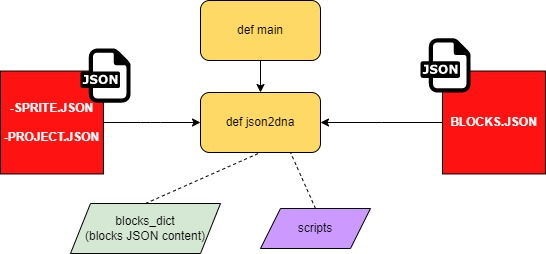
\includegraphics[width=13cm, keepaspectratio]{img/flow_statistics.jpg}
  \caption{Diagrama de funcionamiento de statistics.py}
  \label{fig:flow_statistics}
\end{figure}

\section{Análisis de datos} 
\label{sec:extracciondatos}

\subsection{cluster.py}

Un algoritmo de clusterización es un método para agrupar objetos de tal manera que los objetos en el mismo grupo (cluster) sean similares entre sí, mientras que los objetos en diferentes grupos (clusters) sean lo suficientemente diferentes.

El algoritmo que se emplea es El algoritmo de propagación de afinidad es un algoritmo de aprendizaje automático que se utiliza para encontrar patrones ocultos en datos no estructurados. Se basa en la idea de que los datos que se parecen a unos pocos puntos de datos son más probable que sean similares a otros puntos de datos. El algoritmo se ejecuta en iteraciones, en cada iteración, se seleccionan algunos puntos de datos y se les asignan etiquetas. Luego, el algoritmo busca otros puntos de datos que se parezcan a los puntos de datos etiquetados y les asigna las mismas etiquetas. El algoritmo continúa iterando hasta que todos los puntos de datos hayan sido etiquetados.


El código de este script importa la función de levenshtein de la biblioteca distance y la función Counter de la biblioteca collections. Luego, define una función llamada json2dna que toma como argumento un archivo JSON y devuelve los scripts como caracteres. En la función main, el código convierte los scripts en una matriz y luego usa la función de levenshtein para calcular la similitud entre los scripts. Finalmente, el código imprime los resultados del clustering.

FALTA POR DESARROLLAR.

\section{Visualización de resultados} 
\label{sec:visualizacionresultados}

Se visualiza en el siguiente formato por línea de comandos:

\begin{lstlisting}[style=consola,numbers=none]
*** STARTING ANALYSIS  ***

-- STARTING DUPLICATESCRIPTS.PY SCRIPT --

Looking for duplicate blocks in (FILENAME)

Minimum number of blocks:  X

XX total blocks found
XX total blocks ignored
XX total scripts found
XX total sprites found
XX intra-sprite duplicate scripts found
XX project-wide duplicate scripts found
XX custom blocks found in all project
XX custom blocks calls found in all project

-- END OF DUPLICATESCRIPTS.PY SCRIPT --


-- GETTING INTRA SPRITE STATISTICS --

10 most common:
XX times
	BLOCK NAME 
	BLOCK NAME
	...

Different blocks: XX


-- GETTING INTRA PROJECT STATISTICS --

10 most common:
XXX times
	BLOCK NAME
	BLOCK NAME
	...


Different blocks: XX


-- STARTING CLUSTER.PY SCRIPT --

(CLUSTERING INFORMATION)

-- END OF CLUSTER.PY SCRIPT --


*** ENDING ANALYSIS  ***


\end{lstlisting}

%Recuerda que toda figura que añadas a tu memoria debe ser explicada.
%Sí, aunque te parezca evidente lo que se ve en la figura~\ref{fig:arquitectura}, la figura en sí solamente es un apoyo a tu texto.
%Así que explica lo que se ve en la figura, haciendo referencia a la misma tal y como ves aquí.
%Por ejemplo: En la figura~\ref{fig:arquitectura} se puede ver que la estructura del \emph{parser} básico, que consta de seis componentes diferentes: los datos se obtienen de la red, y según el tipo de dato, se pasará a un \emph{parser} específico y bla, bla, bla\ldots

%Si utilizas una base de datos, no te olvides de incluir también un diagrama de entidad-relación.


%%%%%%%%%%%%%%%%%%%%%%%%%%%%%%%%%%%%%%%%%%%%%%%%%%%%%%%%%%%%%%%%%%%%%%%%%%%%%%%%
%%%%%%%%%%%%%%%%%%%%%%%%%%%%%%%%%%%%%%%%%%%%%%%%%%%%%%%%%%%%%%%%%%%%%%%%%%%%%%%%
% EXPERIMENTOS, VALIDACIÓN Y RESULTADOS%
%%%%%%%%%%%%%%%%%%%%%%%%%%%%%%%%%%%%%%%%%%%%%%%%%%%%%%%%%%%%%%%%%%%%%%%%%%%%%%%%

\cleardoublepage
\chapter{Experimentos, validaciones y resultados}

%Este capítulo se introdujo como requisito en 2019. 
%Describe los experimentos y casos de test que tuviste que implementar para validar tus resultados. 
%Incluye también los resultados de validación que permiten afirmar que tus resultados son correctos. 

Hablar de la pruebas de escalabilidad. 

FALTA POR DESARROLLAR.

%%%%%%%%%%%%%%%%%%%%%%%%%%%%%%%%%%%%%%%%%%%%%%%%%%%%%%%%%%%%%%%%%%%%%%%%%%%%%%%%
%%%%%%%%%%%%%%%%%%%%%%%%%%%%%%%%%%%%%%%%%%%%%%%%%%%%%%%%%%%%%%%%%%%%%%%%%%%%%%%%
% CONCLUSIONES %
%%%%%%%%%%%%%%%%%%%%%%%%%%%%%%%%%%%%%%%%%%%%%%%%%%%%%%%%%%%%%%%%%%%%%%%%%%%%%%%%

\cleardoublepage
\chapter{Conclusiones}
\label{chap:conclusiones}

Cuando empecé a aprender a programar en Scratch, una de las cosas que me llamó la atención fue la facilidad con la que se podía duplicar código. Al principio, no entendía realmente la importancia de esto, pero a medida que seguía aprendiendo más sobre este lenguaje, empecé a darme cuenta del impacto que esto podría tener en el desarrollo de la abstracción. La razón por la que el código duplicado es un problema en Scratch es porque es un lenguaje de programación visual. Esto significa que el código no se escribe en texto, sino que se crea encajando bloques de código. Esto hace que sea muy fácil duplicar código por accidente.

La abstracción es el proceso de ocultar complejidad detrás de una interfaz más simple. En Python, esto se consigue normalmente creando funciones o clases. Al abstraer los detalles de una parte concreta del código, hacemos que sea más fácil de entender y reutilizar. En Scratch, es un poco más complicado ya que la propia interfaz nos limita la reutilización de custom\_blocks. Por ejemplo, si creamos una función elemental en el objeto ''personaje'', solamente podremos utilizarla dentro de dicho objeto, obligando a crear nuevamente la función para tantos objetos como se desee la implementen.

Por otro lado, el código duplicado es el que se repite varias veces en un programa. Esto puede ser un gran problema para la mantenibilidad, porque si necesitamos cambiar el código, tendremos que cambiarlo en múltiples lugares, u objetos en este caso. Esto también puede conducir a errores si el código no se actualiza correctamente.

También se ha podido comprobar en la literatura científica~\cite{baxter_yahin} que los proyectos de Scratch hacen uso extensivo del clonado lo cuál puede suponer una limitación a la hora de desarrollar habilidades del pensamiento computacional, especialmente, la abstracción.

FALTA POR DESARROLLAR.

\section{Consecución de objetivos}
\label{sec:consecucion-objetivos}

%Esta sección es la sección espejo de las dos primeras del capítulo de objetivos, donde se planteaba el objetivo general y se elaboraban los específicos.

%Es aquí donde hay que debatir qué se ha conseguido y qué no. 
%Cuando algo no se ha conseguido, se ha de justificar, en términos de qué problemas se han encontrado y qué medidas se han tomado para mitigar esos problemas.

%Y si has llegado hasta aquí, siempre es bueno pasarle el corrector ortográfico, que las erratas quedan fatal en la memoria final.
%Para eso, en Linux tenemos aspell, que se ejecuta de la siguiente manera desde la línea de \emph{shell}:

%\begin{verbatim}
%  aspell --lang=es_ES -c memoria.tex
%\end{verbatim}

FALTA POR DESARROLLAR.

\section{Conocimientos aplicados}
\label{sec:aplicacion}

%Aquí viene lo que has aprendido durante el Grado/Máster y que has aplicado en el TFG/TFM. Una buena idea es poner las asignaturas más relacionadas y comentar en un párrafo los conocimientos y habilidades puestos en práctica.

La capacitación y el desarrollo de los conocimientos son fundamentales para el éxito en cualquier ámbito. A menudo, se asume que el conocimiento es una habilidad innata que se adquiere a través de la experiencia y el aprendizaje. Sin embargo, el conocimiento también puede adquirirse a través de la capacitación y el desarrollo de estas habilidades.

Durante el transcurso del grado, me percate que el éxito requiere de una combinación de capacitación, desarrollo de los conocimientos y experiencia. Esto es ciertamente aplicable a todas las habilidades que he desarrollado a lo largo de estos años. Quiero enumerar, por asignaturas, dichas habilidades aprendidas y que han facilitado realizar este trabajo.

\begin{enumerate}
  \item Protocolos para la Transmisión de Audio y Vídeo en Internet
\end{enumerate}

FALTA POR DESARROLLAR.

\section{Conocimientos aprendidos}
\label{sec:aprendizaje}

FALTA POR DESARROLLAR.


\section{Trabajos futuros}
\label{sec:trabajos_futuros}

%El programa tiene un amplio rango de mejora a nivel de código y escalabilidad. 
FALTA POR DESARROLLAR.


%Ningún proyecto ni software se termina, así que aquí vienen ideas y funcionalidades que estaría bien tener implementadas en el futuro.

%Es un apartado que sirve para dar ideas de cara a futuros TFGs/TFMs.

%%%%%%%%%%%%%%%%%%%%%%%%%%%%%%%%%%%%%%%%%%%%%%%%%%%%%%%%%%%%%%%%%%%%%%%%%%%%%%%%
%%%%%%%%%%%%%%%%%%%%%%%%%%%%%%%%%%%%%%%%%%%%%%%%%%%%%%%%%%%%%%%%%%%%%%%%%%%%%%%%
% BIBLIOGRAFIA %
%%%%%%%%%%%%%%%%%%%%%%%%%%%%%%%%%%%%%%%%%%%%%%%%%%%%%%%%%%%%%%%%%%%%%%%%%%%%%%%%

\cleardoublepage

% Las siguientes dos instrucciones es todo lo que necesitas
% para incluir las citas en la memoria
\bibliographystyle{ieeetr}
\bibliography{memoria}
% memoria.bib es el nombre del fichero que contiene
% las referencias bibliográficas. Abre ese fichero y mira el formato que tiene,
% que se conoce como BibTeX. Hay muchos sitios que exportan referencias en
% formato BibTeX. Prueba a buscar en http://scholar.google.com por referencias
% y verás que lo puedes hacer de manera sencilla.
% Más información: 
% http://texblog.org/2014/04/22/using-google-scholar-to-download-bibtex-citations/

%%%%%%%%%%%%%%%%%%%%%%%%%%%%%%%%%%%%%%%%%%%%%%%%%%%%%%%%%%%%%%%%%%%%%%%%%%%%%%%%
%%%%%%%%%%%%%%%%%%%%%%%%%%%%%%%%%%%%%%%%%%%%%%%%%%%%%%%%%%%%%%%%%%%%%%%%%%%%%%%%
% APÉNDICE(S) %
%%%%%%%%%%%%%%%%%%%%%%%%%%%%%%%%%%%%%%%%%%%%%%%%%%%%%%%%%%%%%%%%%%%%%%%%%%%%%%%%

\cleardoublepage
\appendix
\chapter{Disponibilidad del código}
\label{app:codigo}

El código del trabajo desarrollado se puede encontrar alojado en el siguiente repositorio de GitHub:

\textbf{https://github.com/felipsandoval/duplicatescripts-scratch}

\chapter{Manual de usuario}
\label{app:manual}

%Esto es un apéndice.
%Si has creado una aplicación, siempre viene bien tener un manual de usuario.
%Pues ponlo aquí.

\textbf{USO}
\begin{lstlisting}[style=consola,numbers=none]
$ python3  program.py  <fichero(.SB3 o .JSON o .ZIP)>  [-i]
\end{lstlisting}

-i (OPCIONAL): Ignora los opcodes de bloques especificados en IgnoreBlocks.txt
\\\\
\textbf{USAGE}
\begin{lstlisting}[style=consola,numbers=none]
$ python3  program.py  <file(.SB3 or .JSON or .ZIP)>  [-i]
\end{lstlisting}

-i (OPTIONAL): Ignores blocks opcodes specified in IgnoreBlocks.txt

\chapter{Requisitos}
\label{app:requisitos}

Para poder hacer uso del programa es importante tener instalado los módulos y bibliotecas de Python necesarias para el funcionamiento del programa,  por ello es necesario ejecutar el siguiente comando:

\begin{lstlisting}[style=consola,numbers=none]
$ pip install -r requirements.txt
\end{lstlisting}

\end{document}
